\documentclass[a4paper,12pt]{book}
\usepackage[latin1]{inputenc}
\usepackage[spanish]{babel}
\usepackage{graphicx}

% \title {Reconocimiento Visual de Instrucciones de un entorno 3D para un Robot Aut�nomo}
% \author {Carlos Le�n \and Jorge Mendoza \and Diego S�nchez}

%\makeindex

\begin{document}

\begin{titlepage}
\begin{figure}
  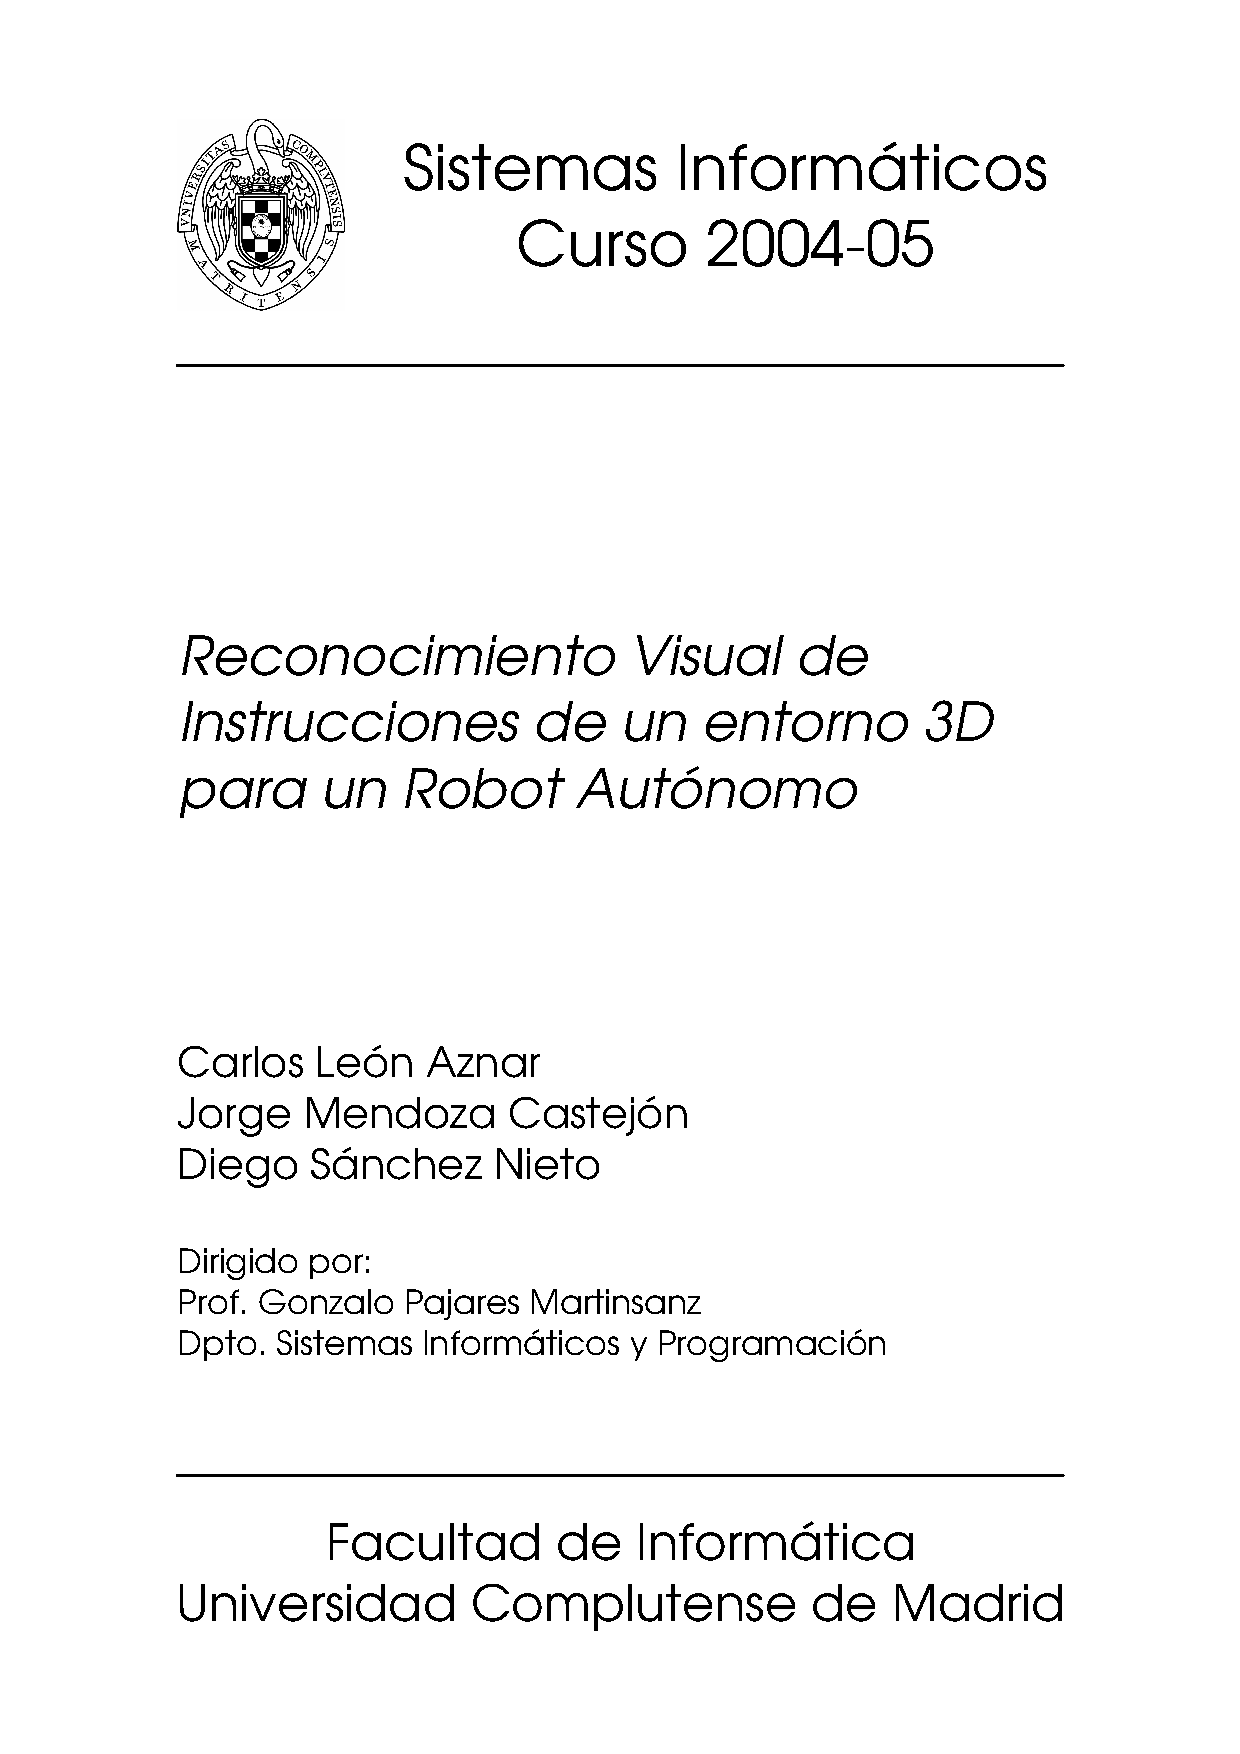
\includegraphics[bb=3cm 0cm 21cm 26cm]{portada.pdf}
\end{figure}
\end{titlepage}


\section*{Resumen del proyecto}

\subsection*{Resumen}
El proyecto consiste en el desarrollo de un motor de visi�n por computador modular, que tiene como objetivo el reconocimiento de gestos de las manos y de �rdenes escritas, adquiridas a trav�s de interfaz de im�genes como una c�mara y otros, y la traducci�n de las mismas a �rdenes inteligibles. Asimismo, se crear�n un microrrobot y un entorno de visualizaci�n en tres dimensiones, que muestren, mediante el movimiento del mismo y el desplazamiento del personaje en el entorno, respectivamente, la ejecuci�n de dichas �rdenes.

\subsection*{Abstract}
The project consists on the development of a modular machine vision engine, that has as objective the reconoissance of hand gestures and written orders, adquired through an image interface like a camera and others, and the translation of these to understandable orders. Also, a micro-robot and a three dimension environment will be created that show, by the movement and the displacement of the character in the environment, respectively, the execution of the mentioned orders.

\subsection*{Palabras clave}
Visi�n, reconocimiento, OCR, neuronal, entorno, 3D, robot, pipeline, m�dulo, imagen.

\section*{Autorizaci�n}
Autorizo a la Universidad Complutense a difundir y utilizar con fines acad�micos, no comerciales y mencionando expresamente a sus autores, tanto la memoria, como el c�digo, la documentaci�n y/o el prototipo desarrollado.
\bigskip
Firmado:


\tableofcontents


\part {Definici�n del proyecto}
\label {definicion}

\chapter {Introducci�n}
\chapter {Introducci�n}

\section{Objetivos}

El objetivo del proyecto consiste desarrollar en un motor modular de visi�n no dependiente del entorno y el reconocimiento de mensajes, a trav�s de las im�genes capturadas desde una c�mara, para la implantaci�n del sistema de �rdenes de un robot. Para la demostraci�n de la funcionalidad se usar�n un entorno en 3D y un robot construido desde cero.

\section{Organizaci�n de la memoria}


\section{Resumen del proyecto}


\section{Especificaci�n}
 
Vamos  a exponer a continuaci�n los requisitos y caracter�sticas que definen el proyecto de Visi�n por Computador que hemos desarrollado. Esta enumeraci�n ha sido la base a partir de la cu�l se ha desarrollado el dise�o y la posterior implementaci�n de cada uno de los m�dulos que constituyen el proyecto. Por tanto describe las funcionalidades que establecimos inicialmente como objetivos que se deb�an satisfacer una vez concluido el proyecto. Posteriormente ser� necesario realizar una serie de pruebas que confirmen que cada uno de las siguientes caracter�sticas han sido implementadas adecuadamente para corroborar el �xito del proyecto. Est�s pruebas se detallar�n de forma exhaustiva en el apartado correspondiente.

\subsection{Interacci�n con una c�mara de video }
Se deber� poder inicializar, configurar y utilizar una c�mara que se comunique con nuestro proyecto suministrando de forma adecuada las im�genes que deber�n ser analizadas.

\subsection{Adquisici�n y tratamiento de las im�genes}
Los datos suministrados por la c�mara deber�n ser modificados convenientemente para ajustarse a un formato �til para su manipulaci�n por parte de nuestro proyecto. Adem�s, ser� necesario que la imagen recibida a trav�s de la c�mara sea tratada mediante una serie de filtros que resaltar�n y corregir�n adecuadamente los elementos necesarios para su posterior an�lisis.


\subsection{Tolerancia a diferentes condiciones de iluminaci�n }

Debido a que se trata con elementos visuales (im�genes de una c�mara de video), es necesario que el sistema sea tolerante a las diferentes condiciones de iluminaci�n que se pueden dar en distintos entornos. Se debe proporcionar una soluci�n a este respecto que permita la pertinente graduaci�n de los procesos de filtrado y correcci�n de im�genes para poder adaptarse a unas condiciones ambientales variables (obviamente siempre dentro de unos m�rgenes m�nimos de iluminaci�n).

\subsection{An�lisis de las im�genes }
Una vez tratadas adecuadamente, las im�genes deber�n ser analizadas para poder determinar si corresponden a un item reconocido por el sistema. El sistema deber� reconocer dos tipos de items: gestos realizados por el usuario que se interpretar�n como comandos de navegaci�n del robot, y textos escritos en carteles.
Los comandos se generar�n a partir de los gestos que el usuario realice con sus dos manos. En cada una de ellas deber� portar unos guantes con unos puntos de color diferenciados para cada mano. Los gestos de una de las manos se interpretar�n como �rdenes de navegaci�n del tipo avanzar, girar o parar mientras que los gestos de la segunda mano se interpretar�n como el grado de intensidad con la que la orden actual debe ser ejecutada. As� se podr� ordenar que el robot gire a la izquierda con mayor o menor velocidad de rotaci�n por ejemplo. En cuanto al texto, deber� estar escrito sobre carteles de un color que destaque en el entorno. El texto podr� consistir en operaciones aritm�ticas sencillas, �rdenes de control para la navegaci�n del robot, o sencillas preguntas sobre datos que el sistema posea en su base de datos. Una vez analizado, el sistema dar� respuesta seg�n la naturaleza del texto de entrada. En caso de tratarse de una operaci�n aritm�tica, se deber� dar la soluci�n del c�lculo. Si se trata de una orden de navegaci�n, se deber� considerar como un comando de movimiento para el robot que deber� comportarse en consecuencia. Y por �ltimo, si se trata de una pregunta, se deber� dar una respuesta coherente a la sem�ntica y formulaci�n sint�ctica de �sta.

\subsection{Simulaci�n del comportamiento del robot seg�n los comandos procesados }
Para poder comprobar el correcto funcionamiento del sistema de reconocimiento de gestos, se deber� utilizar un sistema que visualice de forma sencilla e intuitiva una simulaci�n del comportamiento que deber�a presentar el robot en respuesta a las �rdenes recibidas. Esta funcionalidad ser� �til tanto para realizar pruebas como para contar con una salida auxiliar que corrobore el comportamiento de un robot f�sico que se conecte al sistema. De esta manera se podr� ir verificando que cada orden procesada es interpretada de forma similar por el robot f�sico en concordancia con lo visualizado en la simulaci�n.

\subsection{Creaci�n y conexi�n al sistema de reconocimiento de un robot }
Se deber� construir un robot mec�nico con capacidades motrices b�sicas (avanzar, retroceder, y girar en ambos sentidos) que se conectar� al sistema de reconocimiento de gestos y actuar� en consecuencia. 



%\section{Estado del arte}


%\section{Punto de partida}

%\section{Conocimientos previos}

%\section{Aportaciones propias}


\subsection{Entornos 3D}

\subsubsection{Introducci�n}

En los �ltimos tiempos se ha producido un avance incre�ble en el desarrollo de aplicaciones que hacen uso de la tecnolog�a gr�fica 3D para representar entornos interactivos que puedan ser explorados por el usuario. En el a�o 1995 se produjo un hito en la tecnolog�a de las tarjetas gr�ficas al aparecer por primera vez en el mercado placas capaces de realizar c�lculos 3D de forma optimizada. Marcas como 3Dfx con su chip Voodoo fueron las pioneras en este sector. Gracias a este avance, se produjo una revoluci�n en el campo de los videojuegos as� como en otros sectores que hac�an uso de los gr�ficos tridimensionales. A partir de ese momento, la escalada en la evoluci�n de los chips gr�ficos fue constantes, habiendo alcanzado hoy en d�a una situaci�n en la que la tecnolog�a (n� de transistores, velocidad de memoria, ancho de banda, etc) de los chips gr�ficos est� a la par e incluso supera a la de los chips principales de un computador(CPU). Sin embargo, esta incremento en la capacidad de c�lculo no hubiera sido suficiente para alcanzar los niveles actuales de realismo en las aplicaciones 3D si no hubiera sido por el desarrollo en paralelo de nuevas soluciones algor�tmicas que aprovecharan este nuevo potencial emergente. De esta manera se han realizado innumerables avances en las t�cnicas de computaci�n gr�fica en campos tan dispares como la representaci�n de terrenos virtuales o las t�cnicas de animaci�n de modelos. Veamos a continuaci�n una breve enumeraci�n de estas nuevas t�cnicas.

\subsubsection{T�cnicas principales}

Terrenos virtuales: El objetivo de todo algoritmo para representar terrenos es la minimizaci�n de la cantidad de tri�ngulos(entidad b�sica  en el procesamiento de geometr�a en 3d) que se deben procesar para mostrar dicho terreno con una calidad y fluidez adecuada. Con este precepto han surgido algoritmos como el CLOD, ROAM, Geometrical MipMapping, VDPM, etc.  Tambi�n es com�n el uso de t�cnicas de partici�n del espacio geom�trico tales como el uso de Octrees, Quadtress, BSP y KD-Trees que permiten optimizar el c�mputo global de los terrenos as� como acelerar los c�lculos de colisiones, etc.

Cielo y Atm�sfera: La representaci�n de la b�veda celeste y de sus elementos (nubes, sol, estrellas, etc) suele realizarse en la mayor parte de los casos utilizando skybox (cubo que engloba el escenario en su interior y que posee una serie de im�genes en cada una de sus caras que representan el cielo),o sky-domes (esferoides truncados sobre los que se texturiza como en el caso anterior una imagen del cielo). Estas t�cnicas se suelen complementar con el uso de capas de texturas animadas para dar dinamismo a las nubes, luces glow para representar el sol o estrellas, e incluso sistemas de part�culas avanzados para conseguir resultados m�s sofisticados como nubes volum�tricas y otros efectos atmosf�ricos como lluvia, niebla, nieve, etc.

Animaciones: Los sistemas de animaci�n de entidades 3D ha evolucionado bastante en los �ltimos a�os. Anta�o las entidades se animaban mediante una t�cnica denominada keyframe. B�sicamente consist�a en grabar a lo largo del tiempo una serie de posiciones (keys) del elemento 3D de forma que posteriormente se interpolaban  para generar una animaci�n.  Posteriormente apareci� el uso de la animaci�n por huesos o esqueleto. En este caso, a la entidad 3d pose�a un esqueleto al c�al iba asociada la piel del modelo. Esta t�cnica increment� sustancialmente el realismo de las animaciones ya que ahora el movimiento produc�a deformaciones coherentes con la morfolog�a de la entidad 3D. Por �ltimo, se complement�  la animaci�n por esqueleto con otras soluciones como el uso de cinem�tica inversa o aplicaci�n de modelos f�sicos(ragdoll) para realizar animaciones que se adaptar�n al entorno virtual en cada situaci�n.

Sombreado: Aunque la iluminaci�n de modelos tridimensionales es algo solventado pr�cticamente desde el nacimiento de la infograf�a, la capacidad de calcular las sombras producidas por un objeto ha sido un problema arduo que a�n hoy en d�a es campo de estudio e innovaci�n. A lo largo de los �ltimo a�os se han generalizado dos t�cnicas principales. La primera se denomina Shadow Mapping y consiste en generar en tiempo real una imagen que contiene las sombras de una escena, para posteriormente proyectar dicha imagen sobre los elementos que son ocluidos por otros respecto a la fuente de luz. La otra t�cnica se denomina Stencil Shadow y hace uso del denominado Stencil Buffer(caracter�stica incorporada en las tarjetas gr�ficas de nueva generaci�n) para calcular las sombras mediante la extrusi�n de la geometr�a del objeto que proyecta las sombras. Este �ltimo algoritmo fue perfeccionado para solucionar ciertas limitaciones mediante una aproximaci�n ideada por John Carmack(presidente de IDSoftware) denominada Z-fail Stencil Shadow.

Sirva la breve descripci�n anterior como ejemplo de la enorme cantidad de innovaciones que se han producido en el campo de la computaci�n gr�fica en los �ltimos tiempos. Nos encontramos inmersos en una etapa de expansi�n constante que la que  cada paso supera con creces los �xitos logrados hasta la fecha. Es por tanto necesario preguntarnos acerca de las futuras tendencias del mundo de la computaci�n 3D.

\subsubsection{Tendencias futuras}

Desde hace poco tiempo se han instaurado en el mercado nuevas tarjetas graficas con P�xel Shaders. Esta nueva tecnolog�a permite el proceso de las im�genes a nivel de p�xel(unidad b�sica que compone cualquier imagen digital). De esta forma, se est� abriendo un nuevo abanico de t�cnicas para elaborar efectos especiales e incrementar de forma asombrosa el foto realismo de las im�genes tridimensionales. Efectos como iluminaci�n por p�xel, normal mapping, parallax mapping,  HDR(High Dymic Range Iluminance), Bloom, Blur, Fressnell Refraction \& Reflexion, y un largo etc�tera que empiezan a aparecer en las nuevas aplicaciones y que a buen seguro colmar�n todas las que aparezcan en el futuro.


\subsection{Redes neuronales}

\subsubsection{Introducci�n}

Desde la aparici�n de las computadoras digitales en los a�os 40 uno de las investigaciones recurrentes ha sido la implementaci�n de sistemas que intentaran simular los procesos cognitivos de los seres humanos. Se ha tratado de crear modelos para reproducir el comportamiento de las neuronas, ya sea de forma individual o en forma de red interconectada por la denominada sinapsis neuronal. Seg�n avanzaba el estudio en el propio campo de la neurolog�a y se iban ampliando los conocimientos sobre las funciones y estructura del cerebro humano, estos modelos simulados fueron evolucionando, aunque no siempre para ajustarse de forma precisa a lo que los nuevos estudios biol�gicos desvelaban. En muchos casos se ha optado por simplificaciones o modificaciones respecto al modelo biol�gico para conseguir una arquitectura pr�ctica a nivel de computaci�n.

\subsubsection{Comienzos}

La nueva tecnolog�a de computaci�n desarrollada a mediados del siglo veinte posibilit� a varios estudiosos la posibilidad de plasmar los conocimientos sobre el proceso de pensamiento humano en modelos de computaci�n. Entre ellos destaca Frank Rossenblant que implement� el Perceptron. Sin embargo pronto se constat� la limitada capacidad del sistema, lo que llev� a que se estableciera un gran pesimismo en este campo de estudio en los a�os venideros.

\subsubsection{Esquemas actuales}

A finales de los a�os 80 hubo un resurgimiento de las redes neuronales, aunque esta vez se prim� la aplicaci�n pr�ctica de esta tecnolog�a por encima de la consecuci�n de un modelo que simulara el comportamiento humano. Se establecieron una serie de arquitecturas para las redes neuronales atendiendo a aspectos como el m�todo de aprendizaje o de entrenamiento. De esta forma existen redes de tipo Hamming o Hopfield(peso fijo), de aprendizaje competitivo o de Mapa de Caracter�sticas(entrenamiento no supervisado), y basadas en decisiones, perceptron, ADALINE, modelos temporales din�micos, etc(entrenamiento supervisado). Gracias a estas nuevas aproximaciones, las redes neuronales se han convertido en una herramienta de uso pr�ctico en multitud de aplicaciones que deben tomar decisiones a partir de c�lculos no deterministas como pueden ser el reconocimiento de im�genes o patrones, predicciones burs�tiles, dise�o de sistemas complejos, etc.

\subsubsection{Futuro}

Parece clara que la tendencia actual de buscar el pragmatismo por encima de la fidelidad en la construcci�n de las redes neuronales se mantendr� en un futuro. Si bien es cierto que el aumento de la capacidad de computaci�n y la previsible revoluci�n que supondr�a la introducci�n de la computaci�n cu�ntica pude hacer que en a�os venideros se retome el objetivo de modelar  el complejo cerebro humano utilizando redes neuronales artificiales.


\subsection{Rob�tica}

\subsubsection{Introducci�n}

El origen de la rob�tica se difumina a lo largo de la historia debido a que se trata de un �rea donde se combinan la ingenier�a industrial, electr�nica, inform�tica, biolog�a, etc, siendo por tanto complejo determinar el momento hist�rico cuando nace como tal esta disciplina. Sin embargo podemos asumir que la aplicaci�n pr�ctica y comercial de los robots se hizo una realidad a lo largo del siglo veinte, gracias entre otros factores a la revoluci�n electr�nica de la miniaturizaci�n y el avance derivado del asentamiento de la inform�tica.

\subsubsection{Evoluci�n}

El objetivo de los robots ha sido inicialmente el de desempe�ar de forma autom�ticas tareas complejas para liberar al hombre de la carga que estas supon�an. Siguiendo esta premisa, el car�cter pr�ctico de la rob�tica ha ido colmando los procesos industriales de aut�matas que han elevado lo que supuso en su momento la revoluci�n industrial a unas cotas de eficiencia y precisi�n que constituyen el pilar fundamental de los procesos de producci�n a gran escala. Este tipo de robots se caracterizan por realizar tareas relativamente simples de una manera sistem�tica y precisa. Normalmente su capacidad sensorial y motriz est�n limitadas para optimizar el desempe�o de sus tareas. Sin embargo, en los �ltimos tiempos otro tipo de robots m�s sofisticados han empezado a ser utilizados satisfactoriamente en tareas mucho m�s complicadas como puede ser la exploraci�n espacial, apoyo log�stico militar, etc. Estas nuevas m�quinas se enfrentan a retos mucho m�s arduos tales como  desenvolverse de forma aut�noma en entornos no controlados. Estas nuevas tareas han impulsado el desarrollo de las capacidades de los robots para analizar y ``comprender'' su entorno, detectar obst�culos, moverse por terrenos no acondicionados, etc.

\subsubsection{Tendencias Futuras}

Los trabajos m�s recientes hacen prever el establecimiento de tres tendencias principales en la rob�tica de aqu� a unos a�os.

El primero, la consolidaci�n de la rob�tica industrial, cada vez m�s sofisticada y eficiente. Sirva como ejemplo el proyecto que se est� desarrollando en la universidad de Southern California consistente en un enorme sistema robot capaz de construir una casa en una �nica jornada de trabajo. De forma aut�noma ser� capaz de recoger el material de construcci�n depositado en la zona de trabajo y en un breve plazo de tiempo levantar muros y paredes siguiendo rigurosamente los planos dise�ados por los arquitectos.

En segundo lugar, seguir�n evolucionando los robots con capacidad para desempe�ar tareas en diferentes tipos de entornos, especialmente en aquellos que constituyen un mayor peligro o incomodidad para los seres humanos. As�  asistiremos al desarrollo de nuevos exploradores espaciales, aeronaves sin tripulaci�n, robots con capacidad para combatir y asistir a tropas del ej�rcito, etc. Sin embargo, es probable que en breve plazo este tipo de aut�matas empiecen a entrar en el �mbito dom�stico en forma de aspiradores aut�nomos, limpiadores de cristales, etc.
Dentro de este grupo parece que se est� estableciendo nuevas perspectivas seg�n las cuales la soluci�n no pasar� por tener un �nico y sofisticado aparato, si no que tareas en principio complejas, ser�n realizadas por multitud de peque�os y simples robots que trabajar�n en equipo. Este camino est� llevando a la emulaci�n de comportamientos biol�gicos de tipo enjambre o colonia como el que se da en algunas especies de insectos. Pongamos por ejemplo el trabajo de los ingenieros de la Universidad Libre de Bruselas, quienes han desarrollado un peque�o robot que simula el comportamiento de una cucaracha. En las pruebas previas, esta peque�a m�quina consigui� infiltrarse en una colonia de estos insectos. En un futuro el objetivo ser� introducir varios ejemplares que consigan destacar como l�deres en la jerarqu�a de la colonia para poder determinar el comportamiento de �sta, haciendo por ejemplo que migren de h�bitat abandonando un lugar de uso humano.

Por �ltimo podemos suponer un amplio desarrollo de los robots en su sentido m�s rom�ntico y m�s presente en la literatura de ciencia ficci�n. Hablamos de la consecuci�n de robots de formas humanoides y con capacidad de interactuar de forma ?inteligente? y ?emotiva? con las personas en su d�a a d�a. En este sentido varios grupos de investigaci�n est�n trabajando desde hace tiempo en un programa a largo plazo que concluya con la fabricaci�n de este tipo de entidades. As� hay que destacar el robot Asimo de Honda, probablemente el aut�mata con la biomec�nica m�s sofisticada desarrollada hasta la actualidad, o los proyectos de universidades como el MIT con Kismet o la de  Carnegie Mellon, cuyos objetivos se centran en desarrollar interfaces sensibles a las emociones humanas para futuras entidades rob�ticas.



\subsection{OCR (Opticar Character Recognition)}

\subsubsection{Introducci�n}

El problema del reconocimiento �ptico de caracteres se trat� por primera vez por parte de la NSA (National Security Agency) estadounidense a principio de los a�os cincuenta. La labor de desencriptar c�digos y mensajes cifrados en aquellos a�os hizo que investigadores como David Sheppard fueran instados a desarrollar un m�todo para reconocer letras de forma autom�tica para su posterior an�lisis criptogr�fico. De esta experiencia previa, surgi� la empresa IMR que en 1955 desarroll� el primer sistema comercial OCR. Una vez traspasado el campo de seguridad gubernamental, la tecnolog�a OCR se implant� en los servicios postales a partir de la d�cada de los a�os sesenta para mejorar los procesos de clasificaci�n del correo.

\subsubsection{Retos de los sistemas OCR}

Cuando tratamos con sistemas del tipo OCR hay que distinguir entre caracteres escritos de forma regular (mediante m�quinas de escribir, imprenta, ordenador, etc) o los escritos a mano.

En el primer caso, el reto de analizar un texto de forma efectiva parece haberse alcanzado con bastante �xito, aunque todav�a quedan ciertos tipos de codificaciones (caracteres no latinos) que presentan ciertos problemas a la hora de ser analizados correctamente por este tipo de sistemas.

En el caso de la escritura a mano, aunque se est�n consiguiendo grandes avances, a�n queda margen para seguir investigando y optimizando los procesos de aprendizaje de los sistemas y la adaptaci�n a las diferentes escrituras de forma individual.

\subsubsection{Futuro}

El futuro de esa tecnolog�a parece discurrir en direcci�n a la consecuci�n de robustos sistemas que permitan, ya no s�lo el an�lisis de un texto, si no la reconstrucci�n de aquellos cuyas caracter�sticas de conservaci�n y antig�edad han hecho que se deterioren provocando que su legibilidad sea harto compleja.


\chapter {Dise�o y arquitectura}
\chapter{Dise�o y arquitectura del proyecto}

\section{Introducci�n}
En este cap�tulo vamos a dar una idea global y poco exhaustiva, pero concreta, de la arquitectura de \emph{Visi�n por Computador}. Tiene dos apartados importantes: la arquitectura modular, y la conexi�n de estos m�dulos.

\section {Arquitectura de la aplicaci�n. M�dulos en tuber�a}
Al dise�ar la aplicaci�n escogimos implementar un sistema altamente modular para conseguir un alto grado de independencia en el desarrollo y de facilidad de ampliaci�n. Por esta raz�n hemos invertido parte del trabajo en desarrollar una plataforma propia de enlace de m�dulos, en la que la una parte de la aplicaci�n (lo que hemos denominado {\em pipeline} o {\em tuber�a}), se encargue de realizar el trabajo mec�nico, que, b�sicamente, se compone de:
\begin{itemize}
\item Conectar los m�dulos mediante puertos independientes con diferente informaci�n por puerto, pudiendo crear conexiones {\em 1 a 1}, {\em n a 1}, {\em 1 a n}, y {\em n a n}.
\item Iniciar y cerrar los m�dulos, creando y liberando la memoria necesaria y llamando a las funciones pertinentes de cada m�dulo.
\item Gestionar un reloj de ciclos de ejecuci�n, transmitiendo la acci�n por el grafo que forma la arquitectura de m�dulos.
\item Control de proyectos de aplicaci�n din�micos, mediante definici�n de los mismos en {\bf XML}. De esta forma, diferentes archivos de configuraci�n de proyecto puden crear aplicaciones totalmente distintas sin tener que reprogramar nada.
\item Manejo de errores mediante retrollamadas a funciones definidas por el usuario.
\end{itemize}
El {\em pipeline} es multiplataforma y funciona con m�dulos compilados desde {\em cualquier lenguaje est�ndar} como bibliotecas din�micas. Esto dota a la aplicaci�n de un marco muy amplio de uso en cualquier �mbito de desarrollo.


\section{Diagrama de pipeline de ``Visi�n por Computador''}
En la figura \ref{diagrama_vision_computador} hemos esquematizado todo el proceso que siguen los datos de nuestra aplicaci�n hasta llegar a una salida visible por el usuario. Los datos comienzan en la interfaz de im�genes (puede ser una imagen de c�mara, un v�deo, una imagen fija...), y descienden por el grafo de m�dulos hasta el \textbf{robot} o el \textbf{entorno 3D}. Asimismo, tenemos tambi�n de entrada las ventanas de par�metros, que dotan a los filtros de los valores necesarios \emph{en tiempo real}.

Tras el filtrado pertinente de cada imagen, se las lleva a un m�dulo de proceso (redes neuronales para los guantes, y algoritmo de \emph{OCR} para el texto), y, paralelamente, a ventanas de visualizaci�n, para depuraci�n y comprobaci�n de resultados. Se filtran las se�ales err�neas y, para el m�dulo de texto, se env�a la informaci�n a un m�dulo de DCG\footnote{Definite clause grammar} que genera una salida como respuesta ``inteligente''. Cuando la informaci�n ya ha sido extra�da de cada imagen, s�lo queda unificarla con el resto de datos, para dar una salida coherente.
%\begin{figure}
%  \label{diagrama_vision_computador}
%  \centering

  %\includegraphics[width=120mm]{pipeline.eps}

  %\caption{Diagrama de tuber�a}
%\end{figure}

\begin{figure}
  \centering
  \includegraphics[width=13.608cm,height=11.404cm,bb=0 0 1113 854]{pipeline.eps}
  \caption{Diagrama de tuber�a}
  \label{diagrama_vision_computador}
\end{figure}





\chapter {Resultados del proyecto}
\section{Pruebas}

\subsection{Pruebas de arquitectura}

\subsubsection{Pruebas de desarrollo}
Uno de los mayores retos del proyecto ha sido conseguir una arquitectura s�lida que satisficiera nuestras necesidades de conexi�n. La evoluci�n de la generaci�n de la aplicaci�n ha llevado impl�citas las pruebas diarias del �xito del dise�o y la implementaci�n de nuestro \emph{pipeline}. Por eso detallamos los cambios del mismo, como resultado de nuestros experimentos.

La primera visi�n del dise�o global era mucho m�s simple que la que finalmente hemos acabado usando: los m�dulos s�lo se conectaban en forma de �rbol. Pronto tuvimos que abandonar este enfoque, pues los requisitos de conexi�n de m�dulos se mostraron m�s complejos de lo que estimamos en un principio.

As� pues, pensamos en conectar los m�dulos \emph{1 a 1} en forma lineal. Los primeros resultados fueron satisfactorios: los m�dulos se comunicaban una vez que la implementaci�n del dise�o dej� de tener errores. La implementaci�n en este punto comenzaba a ser s�lida, y pronto ampliamos el dise�o para que los m�dulos tuvieran conexiones de \emph{1 a N}. Con esto conseguimos, por ejemplo, ver las im�genes que generaban los filtros sin tener que cambiar en absoluto los m�dulos que operaban. El dise�o comenzaba a dar sus frutos, empez�bamos a ahorrar horas de trabajos y a reutilizar fuertemente el c�digo desarrollado, ya que un m�dulo de ``ventana de im�genes'' pod�a, instanci�ndose varias veces, presentar diferentes im�genes.

El dise�o ya comenzaba a ser realmente s�lido, sin embargo, nos vimos en la necesidad de que un m�dulo aceptase varias entradas. Por tanto, a�adimos esa funcionalidad. En esta fase del dise�o completamos casi toda la aplicaci�n. Las pruebas y la correcci�n de errores fueron paralelas y terminaron por dar con un conjunto muy fiable, con conexiones \emph{N a N}.

En �ltima instancia, nos dimos cuenta de que el sistema de puertos no era del todo completo. Un m�dulo s�lo se pod�a conectar a otro por un puerto. Esto nos presentaba el inconveniente en el m�dulo de c�lculo de respuesta, que deb�a ofrecer la salida de la orden y el par�metro de forma independiente. Finalmente, pues, a�adimos m�s potencia a los puertos, dotando a la estructura de una completitud amplia y s�lida.

Como ejemplo global de pruebas y de la utilidad de la arquitectura de \emph{pipeline}, podemos rese�ar el del m�dulo de ``gesti�n''. Poco valorado al principio, pensamos que iba a ser un simple tr�mite de la salida global. Sin embargo, finalmente el diagrama total tiene 4 instancias del m�dulo, para las cuales no hemos tenido que reprogramar nada, s�lo variar el archivo de proyecto XML.

\subsubsection{Eficiencia}

El \emph{pipeline} no es un ejemplo de velocidad de proceso. Las pruebas que hemos realizado nos han permitido, en un ordenador con un microprocesador \emph{Intel Pentium IV} con una frecuencia de reloj de $3.0$ GHz, alcanzar velocidades de ciclo de 200 milisegundos. Para una aplicaci�n del �mbito docente como es la que presentamos, el resultado es desde luego m�s que suficiente, pero no deja de ser un tiempo de ejecuci�n lento para requisitos como, por ejemplo, de tiempo real.

\subsubsection{Comprobaci�n de los m�dulos}
A continuaci�n detallamos las pruebas del aspecto arquitect�nico de los m�dulos:
\begin{itemize}
\item \textbf{Generaci�n im�genes y ventana de im�genes}: El resultado esperado de este m�dulo era la generaci�n de im�genes desde diversas fuentes, en un formato unificado. Para esto, usamos principalmente la ventana de im�genes, comprobando que las im�genes correspondiesen a lo esperado. Para ejemplos de resultados, puede remitirse a la secci�n \ref{imagenes_ejemplos_graficos}.

\item \textbf{Filtros}: La serie de transformaciones que sufre la imagen en el m�dulo de filtro (gestos o carteles) es el resultado de un largo periodo de investigaci�n sobre im�genes de prueba.

La elecci�n de una transformaci�n u otra ha estado dirigida siempre con el prop�sito de conseguir un an�lisis posterior mucho mas simple y fiable.

Todos los filtros que fuimos creando que no presentaban valor a�adido han sido eliminados, quedando as� los m�nimos necesarios para facilitar la extracci�n de informaci�n de la imagen en el posterior an�lisis (red neuronal, OCR).

La elecci�n del tama�o de las mascaras utilizadas o la creaci�n de varios filtros dentro de los mismos bucles se ha realizado siempre con la intenci�n de que la fase de filtro sea lo mas r�pida posible, no impidiendo que la aplicaci�n funcione en tiempo real.

\bigskip
Tiempo aproximado del filtro de gestos:  5 milisegundos.

Tiempo aproximado del filtro de carteles: 6.5 milisegundos.

\item \textbf{Par�metros}: El m�dulo de generaci�n de par�metros tuvo algunos inconvenientes. En un principio, hicimos un programa con el c�digo base de lo que iba a ser el m�dulo, consistente en una ventana que generaba estructuras de datos con los valores elegidos. El funcionamiento del programa fue exitoso, cosa que vimos imprimiendo por pantalla el contenido de dichas estructuras. Cuando integramos el m�dulo (ya programado como tal) en la aplicaci�n, tuvimos algunos problemas, pues los mensajes no llegaban bien al m�dulo de filtros. Las pruebas nos llevaron a la conclusi�n de que fue un fallo de arquitectura, con lo que tuvimos que remodelar el dise�o del n�cleo del pipeline para que admitiese m�s tipos de conexiones. Tras esto, el resultado fue satisfactorio.

\begin{figure}[h]
  \centering
  \includegraphics[scale=0.4]{parametros.png}
  \caption{Pruebas satisfactorias de los par�metros}
\end{figure}

\item \textbf{OCR}: Ha sido uno de los principales retos de este proyecto. Al principio pensamos en utilizar un OCR ya implementado, pero ten�a el problema de que no se ajustaba completamente a nuestras necesidades. Probamos a implementarlo nosotros con algoritmos ya realizados, como descriptores de regiones, pero esos sistemas resultaban ser demasiado lentos cuando el numero de caracteres a reconocer dentro de la imagen aumentaba y como siempre el tiempo ha sido un factor que ha corrido en nuestra contra. Llegamos a plantearnos usar la red neurnal tambien en este campo, pero comprobamos que su entrenamiento era muy costoso, adem�s que no cumplia con las exigencias como por ejemplo que el tama�o de los caracteres no importe. Desarrollamos por tanto nuestro propio algoritmo descriptor reconocedor de caracteres basado en descripci�n de fronteras. La cantidad de informaci�n que este m�todo necesita para describir la frontera de un objeto es muy peque�a lo que acelero todo el proceso. Si queremos que sea muy preciso y que nunca se equivoque reconociendo un objeto aumentamos la cantidad de informaci�n que debe tratar, esto aumenta el tiempo ligeramente, as� que en vez de hacer eso decidimos usar a la salida del OCR un diccionario que comprobara si las palabras que sal�an ten�an o no sentido, si no lo ten�an las correg�a.
\item \textbf{Gesti�n de mensajes}: La gesti�n de mensajes fue probada a trav�s de su funcionamiento, y mostrando la salida por consola. La comprobaci�n de la correcci�n la hemos realizado imprimiendo por la salida est�ndar el estado del grafo de mensajes en todo momento.
\item \textbf{Post-gesti�n de �rdenes}: El m�dulo de gesti�n total de la tuber�a de �rdenes ha tenido pruebas triviales, debido a su sencillez, simplemente, hemos certificado mediante el uso que las �rdenes llegaban bien a los m�dulos de salida.
\item \textbf{Proceso de texto}: El proceso de texto ha sido implementado en Prolog, por lo que las pruebas han sido realizadas de una manera externa a la aplicaci�n, con el int�rprete de SWI-Prolog. Gracias a este m�todo, el desarrollo fue m�s r�pido, ya que la comprobaci�n conun int�rprete es muy �gil. Cuando funcion� por separado, la integraci�n en la aplicaci�n principal no caus� ning�n problema, y funcion� tal y como lo hab�amos previsto, con lo que no hizo falta realizar m�s pruebas que la pura comprobaci�n del funcionamiento en ejecuciones normales. Podemos ver un ejemplo en \ref{pruebas_proceso}.

\begin{figure}[h]
  \centering
  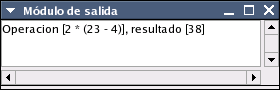
\includegraphics[scale=0.5]{pruebas_texto.png}
  \label{pruebas_proceso}
  \caption{Proceso de texto}
\end{figure}

\item \textbf{Robot}: El desarrollo del robot tuvo un trabajo paralelo. Al principio, las pruebas fueron paralelas a la construcci�n de la estructura, y control�bamos los motores mediante un control de corriente cont�nua. Las pruebas nos llevaron a la conclusi�n de que hab�a que remodelar los �rboles de engranajes y los cambios de par, pues en un principio no suministraban la suficiente potencia como para mover todo el peso de la estructura. Tuvimos que cambiar esto, y fue un cambio bastante grande. Una vez que el robot se mov�a con el control remoto, probamos a crear el circuito que iba a hacer de capa entre el puerto paralelo y los motores. Conectamos el circuito, y sobre la placa las tensiones funcionaban bien. Lo ensamblamos al robot, y, aunque en un principio funcionaba bien, pronto dej� de hacerlo. Tras depurar, vimos que hab�a un fallo en un punto de la placa (nos cost� bastante averiguarlo), y, una vez corregido esto, el robot comenz� a funcionar de una manera muy estable.
\item \textbf{Red neuronal}: Las pruebas sobre la red fueron realizadas antes de empezar el proyecto. Se realizaron pruebas sobre cientos de fotos para el reconocimiento de ciertos patrones, para ello implementamos un peque�o programa de entrenamiento donde contabilizamos el �ndice de aprendizaje sobre el conjunto de fotos de entrenamiento, el �ndice de fallos que comet�a sobre otro conjunto de prueba y sobre otro de validaci�n. Se contabilizaba tanto el �ndice de aciertos como de error, modificando el factor de aprendizaje, el conjunto de entrenamiento y el numero de iteraciones.

\bigskip
Concretamente para el reconocimiento de los 4 gestos que se hacen con la mano al robot se necesitaron 148 fotos de entrenamiento, 49 fotos de validaci�n, 30 de prueba y 20 vueltas de aprendizaje, esto equivale en un Pentium4 a 3 horas de aprendizaje ajustando los pesos de la red.

Porcentaje de aciertos en entrenamiento: 89   Error medio: 0,0141046521582562

Porcentaje de aciertos en validaci�n: 93    Error medio: 0,00799933215976971

Porcentaje de aciertos en prueba: 100     Error medio: 0,00645778571591585v

\begin{figure}[h]
  \centering
  \includegraphics[scale=0.4,bb=0 0 504 231]{Grafica_Aciertos.png}
  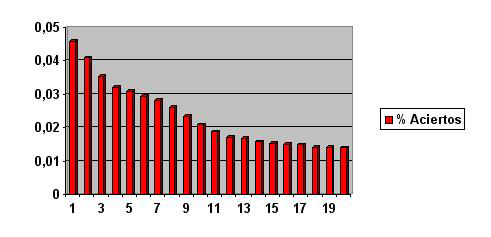
\includegraphics[scale=0.4,bb=0 0 491 237]{Grafica_Errores.png}
  \caption{ La imagen de la izquierda muestra como aumenta el aprendizaje cuanto mas se ense�a a la red. Aumentando el n� de aciertos. Y la de la derecha muestra como a medida que aprende comete menos errores reconociendo figuras.}
\end{figure}

Una vez guardados los pesos en un archivo solo hay que cargarlos en una nueva red cada vez que se quieran utilizar y la retropropagaci�n para el reconocimiento de futuros patrones es casi instant�nea, que es lo que realmente importa. La eficiencia de la red reconociendo patrones es mejorada por el uso de los filtros previos.

\item \textbf{Entorno 3D}: Inicialmente la simulaci�n 3D se prob� exahustivamente de forma aislada para cetificar el correcto funcionamiento de cada uno de los elementos especificados(movimiento del robot, seguimiento de la c�mara, iluminaci�n, etc). En dichas pruebas se utiliz� una entrada directa por teclado gestionada internamente por la aplicaci�n para controlar la navegaci�n del robot a trav�s del escenario. A la hora de realizar la integraci�n con el resto de m�dulos, simplemente se sustituy� el control por teclado interno por los comandos recibidos a trav�s de los puertos de conexi�n resultantes de los an�lisis previos de los gestos del usuario. Una vez establecida la conexi�n del m�dulo con el pipe, s�lo hubo que probar que cada uno de los comandos analizados produc�an el comportamiento deseado en la simulaci�n.Adem�s, como elemento redundante se a�adi� una salida en texto que mostrara al usuario el comando en ejecuci�n en un instante determinado.
\begin{figure}[h]
  \centering
  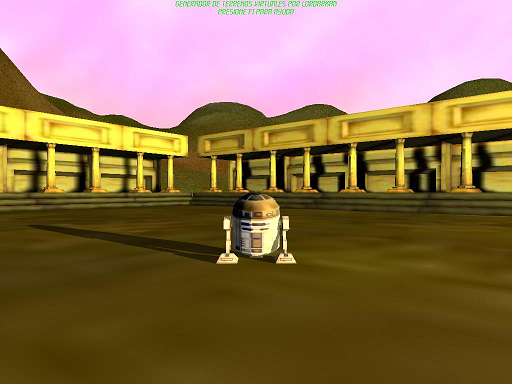
\includegraphics[scale=0.5]{templo1.png}
  \caption{Entorno 3D}
\end{figure}
\item \textbf{Salida de texto}: Para las pruebas de la salida de texto simplemente hemos comprobado que el texto que mand�bamos al m�dulo sal�a por la ventana, a�adimos un ejemplo en la figura \ref{pruebas_salida}.

\begin{figure}[h]
  \centering
  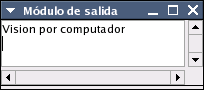
\includegraphics[scale=0.5]{salida_texto.png}
  \label{pruebas_salida}
  \caption{Salida de texto}
\end{figure}

\item \textbf{Joystick}: La comprobaci�n del m�dulo de joystick se ha ido haciendo a medida que la integraci�n avanzaba. Al ser un m�dulo que se ha desarrollado en la fase final de la aplicaci�n, la estructura de la misma ya estaba bastante s�lida, y el funcionamiento del m�dulo ha sido casi inmediato.
\end{itemize}

\chapter{Trabajo futuro}

Dada la extensi�n del proyecto y que concierne a varios �mbitos de desarrollo, vamos a dividir esta secci�n seg�n los apartados del mismo:

%% TODO: Que cada uno ponga aqu� lo suyo. No nos extendamos. Est� ahora liado, pero ya lo estableceremos mejor. No nos preocupemos por las secciones y eso.
\section {No s� qu� poner}

\subsection{La aplicaci�n y los m�dulos}
Los m�dulos de la aplicaci�n son la parte m�s interesante del trabajo posterior al que puede dar lugar este proyecto. Cada uno es independiente de los dem�s, y s�lo ``conocen'' entre s� las interfaces de entrada/salida que los definen. Por tanto, cualquiera de estos m�dulos puede ser incluido en un proyecto de visi�n por computador (en un principio, algunos m�dulos tienen una funcionalidad m�s general). Adem�s, la aplicaci�n que hemos creado puede sera ampliada a�adiendo m�s m�dulos (para crear un sistema m�s inteligente, y enlazar esos nuevos m�dulos con la salida ya existente), o sustituyendo algunos, por ejemplo.


\subsection{Pipeline}

El pipeline consiste en una librer�a en C que conecta m�dulos y pasa informaci�n entre ellos. De este modo, s�lo es necesario crear dichos m�dulos, conectarlos (escribiendo un archivo en \emph{XML}) y establecer sus argumentos (en el \emph{XML} tambi�n). Por tanto, esta pieza de c�digo es perfectamente reusable en cualquier aplicaci�n que necesite una arquitectura modular de elementos independientes que necesiten ser conectados entre s�. 
  
Por otro lado, podr�a tener inter�s la creaci�n, como proyecto futuro, de un editor visual de dichos esquemas de conexi�n de m�dulos, que generase y leyese documentos en XML para el pipeline.

\subsection{Robot}
Mediante la construcci�n del robot hemos demostrado la simpleza de la interacci�n entre software y hardware muy cercano al usuario. Los m�dulos y las rutinas que hemos desarrollado pueden servir bien como ejemplo o base para nuevos proyectos, o como m�dulos ya escritos que pueden ser usados mediante el \emph{pipeline}.

\section{Entorno 3D}:

A continuaci�n se enumeran una serie de ampliaciones y mejoras que se podr�an introducir en el entorno 3d en futuras expansiones del proyecto:

\subsection{Detecci�n de colisiones entre el robot y el entorno}
Se deber�a implementar un sistema para calcular en cada instante la posici�n del punto de contacto del robot con el terreno sobre el que se encuentra. De esta forma el robot podr�a navegar a trav�s de entornos que contasen con suelos accidentados. Adem�s de deber�a calcular posibles colisiones con distintos elementos como paredes, obst�culos y cualquier otro tipo de entidad f�sica que se encuentre dentro de la simulaci�n.

Para implementar la opci�n de que el robot se desplace sobre una superficie abrupta, se sugiere implementar un sistema que a partir de las coordenadas XZ del robot, se obtenga la correspondiente altura del terreno en ese punto, es decir la coordenada Y, la cual servir� para situar al robot a la altura adecuada. Este c�lculo es trivial y consiste en una simple interpolaci�n entre los v�rtices que componen el tri�ngulo en cuyo interior se encuentra el punto XZ proyectado sobre el plano hom�nimo. Para realizar estos c�lculos es necesario acceder a la informaci�n geom�trica del terreno. Dicha informaci�n es accesible de una forma simple a trav�s de la clase Terreno que se ha implementado.

En el caso de las colisiones con otros elementos del entorno lo m�s sencillo ser�a implementar un sistema de colisiones jer�rquico. Este sistema consiste en ir realizando diferentes test de colisi�n que, de forma gradual, fueran refinando la precisi�n del c�lculo de la colisi�n. De esta forma, se empezar�a por realizar un test de colisi�n entre las bounding box (cajas imaginarias que engloban el volumen de una entidad 3d) del robot con los diferentes objetos est�ticos del entorno. Si no existe colisi�n a este nivel, podemos asegurar que no hay colisi�n y por tanto terminar en este punto el c�lculo. Si se produce colisi�n entre diferentes bounding box, debemos asegurarnos de que verdaderamente la geometr�a contenida en las cajas est�n en contacto. Para ello se pasar�a a un segundo test de grano mucho m�s fino, en el que se realizar�an comprobaciones de colisi�n entre los tri�ngulos de cada una de las entidades 3d implicadas en la colisi�n. Este �ltimo c�lculo suele ser bastante costos en cuanto a tiempo de computaci�n, por eso es importante descartar en una primera pasada todas las situaciones que no requieran un c�lculo tan preciso. De nuevo, la clase Objeto proporcionada, da acceso a todos los datos de la geometr�a necesarios para realizar estos c�lculos. Adem�s, el propio lenguaje gr�fico empleado (Direct3D), proporciona a trav�s de su librer�a auxiliar D3DX multitud de funciones que facilitan la implementaci�n del sistema de colisiones aqu� propuesto.

A�adiremos una �ltima cuesti�n respecto al tema de las colisiones. Si se quisiera representar un entorno extremadamente complejo, con una gran cantidad de geometr�a 3d, ser�a necesario a�adir un nivel m�s a la jerarqu�a de colisiones previamente expuesta. Ser�a adecuado realizar en primera instancia un test previo en el cu�l se detectar�a en que sector del escenario se encuentra el robot, pudiendo descartar en esta primera pasada todos aquellos elementos que se encontrar�n fuera de dicho sector. Luego se pasar�a a realizar el algoritmo ya explicado �nicamente con los objetos que comparten sector con el robot. Para implementar este sistema, habr�a que crear una estructura de partici�n del entorno. Se pueden optar por distintas aproximaciones como el uso de �rboles BSP, Octrees, Quadtrees, etc. Sobre estas estructuras existe multitud de documentaci�n al ser algoritmos de uso com�n en computaci�n gr�fica.

\subsection{Creaci�n de rutas de navegaci�n}
Para demostrar la funcionalidad del sistema de visi�n por computador como sistema de control de un robot, se podr�an establecer diferentes rutas en el entorno 3d, que el robot debe seguir guiado por el usuario. De esta forma, el usuario deber�a guiar al robot a lo largo de una serie de puntos de control o waypoints para completar un recorrido. Adem�s se podr�a incrementar la dificultad de dicho reto imponiendo reglas como recorrer la ruta en un tiempo determinado o a una velocidad lineal o de giro m�nima.

La implementaci�n de esta ampliaci�n ser�a trivial una vez implementado el sistema de colisiones previamente propuesto. As�, simplemente habr�a que disponer una serie de objetos que se corresponder�an con los puntos de navegaci�n e ir comprobando si el robot colisiona con ellos en el orden adecuado. Obviamente habr�a que inhibir cualquier respuesta motriz a dicha colisi�n, ya que estos objetos no deber�a impedir el movimiento del robot.

\subsection{Modificaci�n de los modelos (Robot, Escenario o Terreno)}. Si se quiere cambiar el aspecto de la simulaci�n, incorporando nuevos modelos para los objetos 3d, simplemente habr�a que convertir los nuevos modelos desde su formato origen (normalmente formatos de programas de modelado 3D como 3Dstudio o Maya) al formato .X que es el que se usa en la aplicaci�n. Dicha conversi�n se puede realizar a partir de los plugins que incluye el SDK de DirectX. Para modificar el terreno, �nicamente hay que crear un nuevo mapa de altura (en formato crudo o RAW) y utilizar la peque�a aplicaci�n auxiliar desarrollada para generar terrenos que configura el tama�o y grado de desnivel de la geometr�a as� como las diferentes capas de texturas que se usar�n en funci�n de la altura.

\subsection{Mejoras en el apartado gr�fico}
Para incrementar el aspecto visual de la aplicaci�n se pueden introducir en el futuro nuevos efectos gr�ficos. Por ejemplo, se podr�a introducir el uso de texturas HDR que optimicen el comportamiento visual de la iluminaci�n y los reflejos de los objetos 3D. Se podr�a incluir tambi�n la novedosa t�cnica PRT(precomputed radiance transfer) que permite implementar la t�cnica de iluminaci�n global por radiosidad en tiempo real (esta caracter�stica se ha incorporado a la nueva versi�n de DirectX aparecida en Abril de 2005). Por supuesto, el uso de shaders para desarrollar nuevos efectos ser�a tambi�n muy apropiado, teniendo en cuenta adem�s lo f�cil de su programaci�n gracias a las facilidades de Direct3D para integrar esta tecnolog�a.

Cualquier otro tipo de modificaci�n ser� f�cilmente implementada ya que el dise�o de la aplicaci�n y su modularidad permiten una sencilla integraci�n de nuevos componentes. Para m�s detalles consultar el dise�o en el Anexo correspondiente al Entorno 3D.



%\section{Conclusiones}


%\section{Agradecimientos}

\begin{itemize}
  \item Gracias a Jos� Antonio L�pez Orozco por su ayuda en la construcci�n del robot.
  \item Gracias a Juan Rodr�guez por su ayuda con el reconocedor en Prolog.
\end{itemize}
%\begin{thebibliography}{10}

\bibitem{PAJARES}
Gonzalo Pajares, Jes�s M. de la Cruz
\newblock ``Visi�n por Computador: Im�genes Digitales y Aplicaciones''
\newblock Ra-Ma.

\bibitem{PAJARES2}
Gonzalo Pajares, Jes�s M. de la Cruz, Jos� M. Molina, Juan Cuadrado, Alejandro L�pez
\newblock ``Im�genes Digitales''
\newblock Ra-Ma.

\bibitem{MITCHELL}
Tom M. Mitchell
\newblock ``Machine Learning''
\newblock McGraw-Hill, 1997.

\bibitem{WITTEN}
Ian H. Witten, Eibe Frank
\newblock ``Data Mining: Practical Machine Learning Tools and Techniques with Java Implementations''
\newblock Morgan Kaufmann, 1999.

\bibitem{RUSSELL}
Russell, S. y Norvig, P.
\newblock ``Artificial Intelligence: A Modern Approach''
\newblock Prentice Hall, 2004.

\bibitem{RICH}
Rich, E. y Knight, K.
\newblock ``Artificial Intelligence''
\newblock McGraw-Hill, 1994.

\bibitem{LUNA}
Frank D.Luna
\newblock ``Introduction to 3D game programming with DirectX 9.0''
\newblock Wordware Publishing, Inc

\bibitem{POLLACK}
Trent Pollack
\newblock ``Focus On 3D Terrain Programming''
\newblock Muska y Lipman/Premier-Trade

\bibitem{SANCHEZ}
Julio Sanchez, Maria P.Canton
\newblock ``DirectX 3D Graphics Programming Bible''
\newblock IDG Books Worldwide,Inc.

\bibitem{ZERBST}
Estephan Zerbst
\newblock ``3D Game Engine Design''
\newblock Premier Press.

\bibitem{ROBO1}
An�bal Ollero
\newblock ``Rob�tica: Manipuladores y robots m�viles''
\newblock Marcombo

\bibitem{ROBO2}
Edwin Wise
\newblock ``Applied Robotics''
\newblock Prompt Publications

\bibitem{ROBO3}
Phillip John McKerrow
\newblock ``Introduction to Robotics''
\newblock Addison-Wesley

\bibitem{ROBO3}
K.S. Fu, R.C. Gonz�lez, C. S. G. Lee
\newblock ``Rob�tica: control, detecci�n, visi�n e inteligencia''
\newblock McGraw-Hill

  
\end{thebibliography}


\part{Detalles de los m�dulos}
\label{anexo1}
\chapter{Filtros}

La visi�n artificial es el proceso sensorial m�s complejo de todos.
Las tareas en vis�n por computador se pueden enumerar en:
\begin{enumerate}
\item Visi�n de bajo nivel. (Tareas autom�ticas)
  \begin{itemize}
  \item Captaci�n. Obtenci�n de la imagen.
  \item Preprocesamiento. Incluye t�cnicas como reducci�n de ruido y realce de detalles.
  \end{itemize} 
\item Visi�n de nivel medio. (Etiquetar objetos)
  \begin{itemize}
  \item  Segmentaci�n. Localizaci�n de los objetos de inter�s.
  \item Descripci�n. Obtenci�n de caracter�sticas: tama�o, formas, etc.
  \end{itemize} 
\item Visi�n de alto nivel. (Emular inteligencia)
  \begin{itemize}
  \item Reconocimiento. Identificaci�n de objetos: tornillos, puertas, etc.
  \item Interpretaci�n. Significado de un conjunto de objetos.
  \end{itemize} 
\end{enumerate} 

El objetivo de los filtros utilizados en nuestro proyecto entra en el �mbito del preprocesamiento y segmentaci�n de im�genes.
Ejemplos de la fase de preprocesamiento son el suavizado, el realce, detecci�n de bordes, detecci�n de umbral, etc.
El procesamiento de una imagen puede ser visto como una transformaci�n de una imagen en otra imagen, es decir, a partir de una imagen, se obtiene otra imagen modificada. Desde el punto de vista de visi�n artificial, el �nico prop�sito del procesamiento de im�genes es conseguir mas adelante un an�lisis de estas mas simple y mas fiable. Por consiguiente, el procesamiento de im�genes debe facilitar la extracci�n de informaci�n para un posterior an�lisis, de manera que la escena pueda ser interpretada de alguna manera.

Por este motivo aplicamos a la imagen capturada por la webcam una serie de filtros, para simplificar la imagen, hasta el punto de eliminar la informaci�n que no nos interesa y realzar la informaci�n importante para el an�lisis posterior de la imagen, en este caso el reconocimiento de gestos y carteles.

Para saber mas sobre im�genes digitales: \ref {Imagen Digital} (p�gina \pageref{Imagen Digital}).

La capacidad visual del robot, depender� de los m�dulos de visi�n que est�n activos. De momento solo hay m�dulos implementados y activos que permiten al robot recibir ordenes con gestos hechos con unos guantes o tambi�n recibir informaci�n procedente de carteles. Los carteles no solo pueden darle ordenes, si no hacerle una pregunta de la cual tenga conocimiento o hacerle realizar una operaci�n aritm�tico-l�gica.

Por tanto los �nicos medios para comunicarse con el robot son guantes y carteles especiales, de momento.

Son especiales por su color. La raz�n de utilizar colores especiales ha sido crear en las im�genes capturadas, regiones de color con unos rangos de intensidades en los tres colores, mas separadas del resto de intensidades del histograma de la imagen. As� podremos aislar esta regi�n, la del color especial. En el caso de los guantes, es la posici�n de los dedos la que indica la orden, es en los dedos donde esta el color especial, as� que si solo nos quedamos con las regiones de este color y el resto lo despreciamos, estaremos simplificando much�simo la imagen para un posterior an�lisis de esta. Lo mismo pasar�a con los carteles, desechamos toda la imagen que no forme parte del cartel y dentro del cartel nos quedamos solo con la frase.

Filtro de guantes. \ref {Filtro de Gestos} (p�gina \pageref{Filtro de Gestos}).
Filtro de carteles. \ref {Filtro de Carteles} (p�gina \pageref{Filtro de Carteles}).

Los m�dulos posteriores a los filtros son m�dulos de an�lisis que deben de recibir la informaci�n lo mas clara posible, en el caso de los gestos se utiliza una red neuronal, la cual tiene que ser entrenada con im�genes muy simplificadas para que el entrenamiento tenga efecto y que las im�genes que reciba una vez entrenada, sean filtradas de la misma manera, para generar im�genes iguales que con las que fue entrenada, para poder reconocerlas. Respecto a los carteles el siguiente modulo es un OCR, muy sensible a ruidos, por tanto hay que asegurar que el filtro es efectivo, para que la salida de este no sea incoherente.


\chapter{M�dulo de generaci�n de im�genes}

\section{Introducci�n}
Este m�dulo tiene como objetivo la creaci�n y modificaci�n de un b�fer de colores (una imagen en formato plano) para la alimentaci�n de la tuber�a de visi�n. Obtiene, de diferentes fuentes, imagenes codificadas de diferentes maneras, y genera, en un formato unificado, una imagen sin comprimir.

\section {Im�genes generadas}
% Hablar de los formatos

\section {Arquitectura y funcionamiento del m�dulo}
El m�dulo sigue las interfaces de comunicaci�n con el {\em pipeline}, de modo que crea los b�feres en la funci�n de iniciar, a la vez que, seg�n se haya instanciado a trav�s de la configuraci�n del XML que define el proyecto, abre la comunicaci�n con las bibliotecas pertinentes, en funci�n de los argumentos.

En el ciclo de im�genes se procede seg�n sea el funcionamiento. En el caso de que las im�genes cambien cada ciclo (no pasa cuando son im�genes de un color fijo o cargadas de archivo), se obtiene del recurso indicado el b�fer en el formato que ofrezca la biblioteca, y se transforma al formato de salida com�n, como se ha comentado en la secci�n anterior. Una vez que se ha hecho esto, se ``deposita'' en el puerto de salida la imagen resultante, habiendo ya dado uniformidad a las diferentes entradas, haciendo que el {\em pipeline} no dependa de las fuentes generadores de im�genes a m�s bajo nivel.

En la funci�n de cerrar simplemente libera los recursos.

\section {Bibliotecas}
Para la generaci�n resultados desde diferentes fuentes, el m�dulo hace uso de una serie de librer�as; son las siguientes:

\begin {itemize}
\item {\bf SANE}: Sane (Scanner Access Now Easy) es una biblioteca originariamente para interfaces con esc�neres, pero ampliada para cualquier dispositivo de im�genes. A trav�s de esta biblioteca accedemos a la c�mara.
\item {\bf Xine}: Xine-lib tiene como objetivo la reproducci�n de archivos de v�deo en varios formatos (los m�s usuales, tambi�n puede aceptar formatos nuevos a trav�s de {\em plugins}). A trav�s de Xine cargamos un v�deo en el m�dulo de im�genes y lo reproducimos.
\item {\bf Gdk}: Usamos Gdk para cargar f�cilmente archivos de im�genes, y usarlos as� como fuentes sencillas de im�gnenes cuyo resultado se conoce.
\item {\bf C�digo propio}: Tambi�n hemos implementado, para pruebas principalmente, las siguientes funcionalidades del m�dulo:
  \begin {itemize}
  \item {\bf Generaci�n de colores planos}: Pintamos todo el b�fer de un color. Es muy �til para comprobar el funcionamiento de los filtros.
  \item {\bf Generaci�n de im�genes aleatorias}: Rellena la matriz de colores con colores al azar, de esta manera vemos c�mo los filtros aceptan o dejan de aceptar los valores.
  \end {itemize}
\end {itemize}

\section {C�digo}
Ver anexo: documentaci�n del m�dulo de im�genes.c, en \ref {imagenes_8c} (p�gina \pageref{imagenes_8c}).

\chapter{M�dulo de red neuronal}
\label{red_neuronal_label} 

\section{Introducci�n}
Las Redes Neuronales Artificiales (ANNs de Artificial Neural Networks) fueron originalmente una simulaci�n abstracta de los sistemas nerviosos biol�gicos, formados por un conjunto de unidades llamadas neuronas o nodos conectadas unas con otras. Estas conexiones tienen una gran semejanza con las dendritas y los axones en los sistemas nerviosos biol�gicos. 

\bigskip 
Una ANN es un gran numero de conmutadores interconectados, donde a las conexiones se les asigna un peso. Este peso ser� fijado durante la fase de aprendizaje. El procesamiento de informaci�n es paralelo distribuido.

\bigskip 
En que tipos de problemas se utilizan:
\begin{itemize}
\item En problemas donde los ejemplos se describen con un gran numero de atributos.
\item Puede haber ruido en los datos.
\item Cuando no se conoce la forma de la funci�n objetivo. Problemas que no tienen un algoritmo especifico para su soluci�n, o cuyo algoritmo es demasiado complejo para ser encontrado. 
\item Cuando es permisible un tiempo de entrenamiento largo.
\item Ejemplos: Reconocimiento del habla, clasificaci�n de im�genes, predicciones financieras, etc.
\end{itemize} 

\begin{figure}[h]
  \centering
  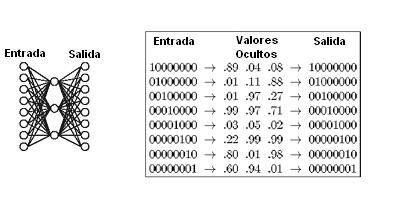
\includegraphics[scale=0.4,bb=0 0 406 203]{red1.png}
  \caption{ Ejemplo esquem�tico de una ANN.}
\end{figure}

\bigskip 
Dicho esto la elecci�n de una red neuronal como medio de resoluci�n del problema de reconocimiento de patrones ser�a en este caso la m�s acertada. Es muy �til cuando no se conoce la funci�n objetivo y se estima que los datos de entrada llegan con cierto porcentaje de ruido. La decisi�n se tom� meses antes de empezar el proyecto. Para asegurarnos de que era viable implementamos la red dentro de un peque�o programa, que a partir de im�genes de entrada devolv�a cierto si detectaba una imagen de una persona con una guante blanco y falso si no hab�a guante.

\section{Descripci�n t�cnica}
Hemos utilizado una red multicapa, ya que permiten representar superficies de decisi�n no lineales. Debido a esto no se puede utilizar unidades lineales ya que solo permitir�an representar funciones lineales. Tampoco pudimos utilizar perceptrones porque su funci�n de salida es discontinua, no derivable y por lo tanto no se le puede aplicar el descenso del gradiente. Necesit�bamos una unidad que diese como salida una funci�n no lineal y que fuese derivable con respecto a las entradas.

\bigskip 
Por eso utilizamos el sigmoide como unidad.

\begin{figure}[h]
  \centering
  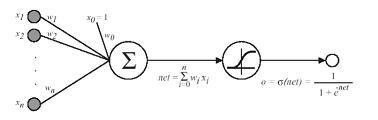
\includegraphics[scale=0.5,bb=0 0 378 120]{red2.png}
  \caption{ Unidad Sigmoide.}
\end{figure}

La funci�n sigma  $ \sigma(x)  = \frac{1}{(1+e^{-x})} $ es no lineal y derivable $ \frac{d\sigma(x)}{dx} =  \sigma(x) . (1 - \sigma(x)) $.

El descenso de gradiente se puede utilizar para entrenar:
\begin{itemize}
\item Una unidad sigmoide.
\item Una red multicapa de unidades sigmoides. Retropropagaci�n.
\end{itemize} 

La retropropagaci�n permite aprender los pesos para una red multicapa con un numero de unidades e interconexiones dado. Consideramos una red con m�ltiples unidades de salida, de forma que el error es la suma de los errores sobre todas las salidas. El espacio de hip�tesis viene dado por los valores posibles para los pesos de todas las unidades de red. Utilizamos el descenso de gradiente para encontrar una hip�tesis que minimice el error, el descenso utilizado es incremental, es decir, los pesos se actualizan despu�s de considerar cada ejemplo de entrenamiento en lugar de esperar a considerarlos todos. Es mas improbable que el descenso incremental caiga en un m�nimo local.
\bigskip 

La secuencia de pasos utilizada en nuestro entrenamiento viene a ser esta:
\begin{itemize}
\item Crear la red. 
\item Se inicializan los pesos de la red con valores peque�os y aleatorios entre -0.05 y 0.05
\item Para una media de 30 iteraciones se realiza lo siguiente: De una lista de im�genes de entrenamiento se va cogiendo una a una y se cargan en la capa de entrada de la red, para esa imagen se calculan las capas, luego seg�n un objetivo se calculo el error cometido en la capa oculta y en la salida y respecto a estos errores se reajustan los pesos de las interconexiones.
\item Se realiza un prueba y una validaci�n con im�genes distintas a las del entrenamiento, para ver el porcentaje de error total cometido, si es aceptable se guarda en un archivo los pesos de la red entrenada, para que en la fase de reconocimiento de im�genes solo haya que realizar el calculo de capas.
\end{itemize} 	

Para cada unidad de salida k, se calcula su termino de error: $ \delta_{k} = O_{k} . (1 - O_{k}) . (t_{k} - O_{k}) $

Para cada unidad oculta h, se calcula su termino de error: $ \delta_{h} = O_{h} . (1 - O_{h}) . \Sigma (W_{kh} . \delta_{k}) $ , siendo k las salidas.

Se actualiza cada peso de la red $ W_{ji} = W_{ji} + \Delta (W_{ji}) $ donde $ \Delta (w_{ji}) = \eta .\delta_{j} .x_{ji} + \alpha .\Delta w_{ji}. (n-1) $. 

($ t_{k} $ es la salida dada por ejemplo de entrenamiento para la unidad k. $ o_{t} $ es la salida generada por la red.)

La actualizaci�n de los pesos en la iteraci�n n depende de la actualizaci�n en n-1. El 2� termino de la ecuaci�n representa la cantidad de movimiento. Un s�mil f�sico seria una pelota que cae por la superficie de error, la cantidad de movimiento hace que la pelota tienda a mantener la misma direcci�n, con esto se intenta evitar que la pelota pare en un m�nimo local o que se pare en un llano.

\bigskip 
Respecto el descenso del gradiente en el sigmoide:
Para el descenso incremental consideramos el cambio en los pesos inducido por cada ejemplo de entrenamiento $ \Delta w_{ji} = \eta \frac{\eta E_{d}}{\eta w_{ji}} $ donde el error sobre un ejemplo de entrenamiento viene dado por la suma de los errores en cada unidad de salida $ E_{d}(w) \equiv \frac{1}{2} . \Sigma (t_{k} - o_{k})^{2} $ , siendo k las salidas

La salida viene dada por $ net = \Sigma w_{i}.x_{i} $ , i=0..n y $ o = \sigma (net) = \frac{1}{1 + e^{-net}} $, aplicando la regla de la cadena $ \frac{\eta E_{d}}{\eta w_{ji}} = \frac{\eta E_{d}}{\eta net_{j}} . \frac{\eta net_{j}}{\eta w_{ji}} = \frac{\eta E_{d}}{\eta net_{j}} . x_{ji} $. Para calcular $ \frac{\eta E_{d}}{\eta net_{j}} $ distinguimos el caso de las unidades de salida y las ocultas.

Error en las unidades de salida $ \frac{\eta E_{d}}{\eta net_{j}} = -(t_{j} - o_{j}). o_{j} .(1 - o_{j}) $. Error en la unidades ocultas $ \frac{\eta E_{d}}{\eta net_{j}} = o_{j} . (1 - o_{j}) . \Sigma (-\delta_{k} . w_{kj})  $.

\bigskip 
Para valores peque�os de los pesos (al principio del proceso) la red presenta una funci�n casi lineal donde es menos probable encontrar m�nimos locales. Cuando la funci�n es mas compleja (un punto mas avanzado del proceso) es de esperar que nos hayamos acercado tanto al m�nimo global que los m�nimo locales sean aceptables. Para garantizar que alcanzamos el m�nimo global utilizamos heur�sticas:
\begin{itemize}
\item A�adiendo cantidad de movimiento.
\item Utilizando descenso incremental.
\item Entrenar distintas redes con los mismos ejemplos, pero con distintos valores iniciales en los pesos.
\end{itemize} 

La capacidad expresiva de este tipo de red es bastante alta ya que:
\begin{itemize}
\item Cualquier funci�n booleana se puede representar con una red de dos capas.
\item Cualquier funci�n continua se puede aproximar con un error arbitrariamente peque�o por una red de dos capas.
\item Cualquier funci�n se puede aproximar con un error arbitrariamente peque�o por una red de tres capas (las dos ocultas de sigmoides y la de salida de unidades lineales).
\end{itemize} 

\section{Dise�o}
Esta formada por una capa de entrada, una de salida y una sola capa oculta.
Si imagin�semos la red como una caja negra, esta tendr�a que recibir como entrada una imagen y sacar como salida una cadena de texto explicativa de alg�n atributo de esa imagen.

\bigskip 
En nuestro caso la entrada ser�n siempre im�genes del mismo tama�o 320x240 p�xeles, por ello la capa de entrada consta de 76800 unidades. En realidad la entrada es un unsigned char* que representa la imagen con valores de 255 o 0, es decir, blanco o negro, recuerdo que las im�genes que le llegan a la red son im�genes que previamente han pasado por el modulo de filtro a si que llegan ya binarizadas. Estas entradas ser�n normalizadas entre 1 y 0, para que las entradas est�n en el mismo rango que las unidades de la capa oculta y de salida.

\bigskip 
La capa oculta debe tener tan pocas unidades como sea posible. Medidas experimentales demuestran que el hecho de aumentar el n�mero de  unidades ocultas proporciona mejoras poco significativas en la precisi�n, pero requieren mucho mas tiempo de entrenamiento. Nosotros hemos optado por utilizar 15 unidades.

\bigskip 
Como ya sabemos al robot se le controla con 2 manos, los gestos de la mano izquierda le indican las ordenes y los de las derecha los par�metros, con el objetivo de simplificar el dise�o los gestos de ordenes y de par�metros son los mismos, pero significan cosas distintas. Tanto para ordenes como para par�metros hay 5 tipos de gestos. Como recordatorio las ordenes eran: parar, avanzar, girar a la izquierda y girar a la derecha. Y los par�metros eran nula, medio baja, medio alta, alta si la orden actual es la de avanzar, donde los par�metros indican la velocidad a la que debe hacerlo o 0�, 45�, 90�, 180� si la orden actual es una de giro. La 5� gesto tanto para ordenes como para par�metros es el ``gesto no reconocido''. Por tanto dado que hay 5 tipos de gestos ha reconocer, la red tendr� que sacar 5 posibles salidas. Al principio optamos por una capa de salida de una sola unidad. El valor oscila entre 0 y 1 as� que por ejemplo si esta unidad val�a 0.2 significaba que hab�a reconocido el 2� gesto, si val�a 0.8 hab�a reconocido el 4� gesto. Luego se cambio al dise�o actual que es una capa de salida de 5 unidades, esto hace a la red mucho mas fiable, se pod�a decir que la salida de la red antes era anal�gica y ahora es digital, ya que todas las salidas tendr�n valores menores de 0.5 excepto una que ser� mayor, solo hay que asociar la unidad de la salida que se ha puesto en alta con una cadena de texto. Esta asociaci�n se hace mediante un script en Lua, as� es m�s modificable ya que si se quiere cambiar el texto de salida no hay que recompilar el proyecto, solo cambiar un archivo de texto.

\bigskip 
La organizaci�n de red por capas es est�ndar, la salida de cada unidad alimenta a todas las unidades de la siguiente capa.

La tasa de aprendizaje utilizada ha sido 0.3. La mas alta posible para reducir el tiempo de aprendizaje sin disminuir la precisi�n.

El descenso de gradiente es incremental para reducir el riesgo de quedarnos en m�nimos locales.

Los pesos de la unidades de salida y oculta son inicializados con peque�os valores aleatorios entre 0.05 y -0.05.

\section{Entrenamiento}
La mayor parte del c�digo utilizado en la red esta dirigido al entrenamiento. Por eso decidimos hacer un programa aparte que contiene el c�digo de entrenamiento de la red y luego el c�digo que est� presente en el proyecto que solo contiene el necesario para crear una red, calcular los valores de las capas a partir del valor de la capa de entrada y generar la cadena de texto de salida. As� el c�digo del proyecto queda mas sencillo para leer.

\bigskip 
El proceso de entrenamiento empieza con la sesi�n fotogr�fica, es necesario hacer mas de un centenar de fotos para obtener un entrenamiento medianamente fiable. Nosotros para el entrenamiento de ordenes sacamos 185 fotos, consiste en sacar fotos d�ndole ordenes al robot correctas, err�neas o simplemente no d�ndoselas. Todas estas fotos han de ser filtradas del mismo modo que lo har�a el modulo de filtro del proyecto, la raz�n de hacer un filtrado previo es poder pasar a la red im�genes muy simples, tambi�n deben de ser tomadas en unas condiciones de iluminaci�n similares a las que tendr� el entorno por el que circule el robot. No es lo mismo hacer aprender a la red a reconocer un gesto perdido en un mar de p�xeles de miles de colores a reconocer un conjunto de p�xeles blancos centrados sobre un fondo negro. Los objetivos mas perseguidos en este proyecto es la eficiencia y en este caso la fiabilidad en el reconocimiento.

\bigskip 
Las fotos son nombradas con un formato determinado, por ejemplo, ``\_orden\_parada\_21.bmp'' esto significa que la foto contiene la orden de parada y ``\_no\_gesto\_51.bmp'' indica que la foto no representa ninguna orden para el robot. Este formato es utilizado en el entrenamiento para que la red sepa ir reajustando los pesos seg�n el nombre explicativo de la foto.

\begin{figure}[h]
  \centering
  \includegraphics[scale=0.5,bb=0 0 160 120]{_no_gesto_36.png}
  \caption{ \_no\_gesto\_36.png}
\end{figure}

Todas las fotos no son utilizadas para el entrenamiento. Se hacen 3 listas de fotos que se utilizaran para el entrenamiento, la prueba y la validaci�n. Estas 2 ultimas sirven  para comprobar el buen funcionamiento de la red entrenada.

El objetivo del programa de entrenamiento es crear una red, entrenarla y salvar la estructura y pesos de red en un archivo.

El entrenamiento consiste en :
\begin{itemize}
\item Recorrer la lista de im�genes de entrenamiento una por una.
\item Cargar la imagen en la imagen en la capa de entrada, cada valor de p�xel se asocia a una unidad de la capa.
\item Seg�n el nombre de la foto, ejemplo ``\_orden\_parada\_21.bmp'', se cambia el objetivo, esto sirve para calcular el error cometido.
\item Cambiado el objetivo, se calcula el valor de la capas respecto a la capa de entrada, se calcula el error cometido en las capas oculta y salida y se reajustan los pesos, para disminuir el error.
\item Esta lista es recorrida un numero finito de iteraciones. Las condiciones de parada pueden ser varias. La nuestra es simplemente un numero concreto, en este caso fueron 30 iteraciones. Por tanto los pesos fueron ajustados 30x(numero de fotos de la lista) veces.
\end{itemize}
Ya tendr�amos as� unos pesos que representan una aproximaci�n a la funci�n buscada.
\bigskip 

\begin{figure}[h]
  \centering
  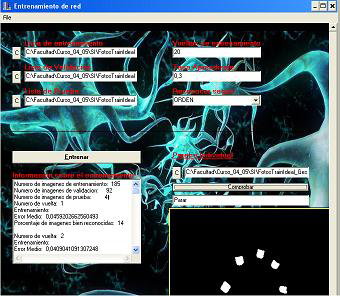
\includegraphics[scale=0.4,bb=0 0 340 296]{prog_train.png}
  \caption{ Captura de nuestro programa de entrenamiento de redes.}
\end{figure}

\bigskip 
Estos fueron datos de un entrenamiento de la red:
\begin{itemize}
\item Datos entrada:
\begin{itemize}
\item 148 fotos de entrenamiento, 49 fotos de validaci�n y 30 de prueba.
\item �ndice de aprendizaje: 0.3
\item 20 iteraciones
\end{itemize} 
\item Datos salida:
\begin{itemize}
\item Porcentaje de aciertos en entrenamiento: 89   Error medio: 0,0141046521582562
\item Porcentaje de aciertos en validaci�n: 93    Error medio: 0,00799933215976971
\item Porcentaje de aciertos en prueba: 100     Error medio: 0,00645778571591585
\end{itemize} 
\end{itemize}   

\begin{figure}[h]
  \centering
  \includegraphics[scale=0.4,bb=0 0 504 231]{Grafica_Aciertos.png}
  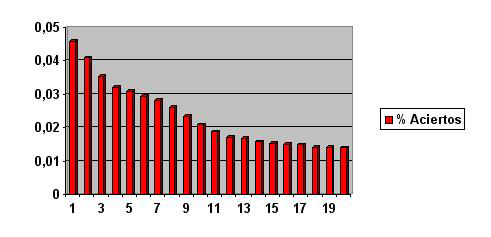
\includegraphics[scale=0.4,bb=0 0 491 237]{Grafica_Errores.png}
  \caption{ La imagen de la izquierda muestra como aumenta el aprendizaje cuanto mas se ense�a a la red. Aumentando el n� de aciertos. Y la de la derecha muestra como a medida que aprende comete menos errores reconociendo figuras.}
\end{figure}

\section{Red Neuronal en el proyecto}
Como cada modulo del pipeline, el modulo de red tiene un peque�o numero de funciones fijas utilizadas para ser llamadas desde el pipeline. Tres de ellas son ``red\_iniciar'', ``red\_cerrar'' y ``red\_ciclo''. Iniciar crea la red y carga el archivo creado por el programa de entrenamiento, por ejemplo el ``orden\_net''. La funci�n cerrar libera toda la memoria. Y la funci�n ciclo lo �nico que hace es recibir un char* que representa la imagen, cargar estos valores normalizados en la capa de entrada y calcular el valor de las capas oculta y de salida seg�n los pesos, que solamente tarda aproximadamente 0.10 segundos. Luego como ya dijimos solamente una de las cinco unidades de la capa de salida tendr� un valor superior a 0.5, esto es equivalente a que se ha puesto en ALTA y el modulo sacar� como salida la cadena de texto asociada a esa unidad. Cadena modificable desde un script junto con el nombre del archivo de la red entrenada. Todo lo que sea modificable en un futuro por posibles mejoras son par�metros que van escritos en scripts.

\bigskip 
Estas son 5 im�genes filtradas de ejemplo, cada una representa una orden o un par�metro.

Recordatorio:
\begin{itemize}
\item 1 dedo: Orden: Avanzar, Par�metro:  Medio baja o 45�
\item 2 dedos: Orden: Girar derecha,  Par�metro:  Medio alta o 90�
\item 3 dedos: Orden: Girar Izquierda,  Par�metro:  Alta o 180�
\item  5 dedos: Orden: Parar ,  Par�metro:  Nula o 0�
\end{itemize} 
 
\begin{figure}[h]
  \centering
  \includegraphics[scale=0.4,bb=0 0 160 120]{_orden_parada_17.png}
  
\includegraphics[scale=0.4,bb=0 0 160 120]{_orden_avanza_38.png}
  
\includegraphics[scale=0.4,bb=0 0 160 120]{_orden_angulo_43.png}
  \includegraphics[scale=0.4,bb=0 0 160 120]{_orden_negAngulo_84.png}
  \caption{ Ejemplos de imagenes de entrada en la red.}
\end{figure}

\section{Evoluci�n}
El primer sistema utilizado para resolver el problema de reconocimiento de gestos, fue la implementaci�n de dos redes distintas una para ordenes y otra para par�metros, debido a que su estructura era distinta.

Se fueron modificando los filtros con el objetivo de facilitar el aprendizaje a la red.

La segunda elecci�n fue utilizar el mismo numero de gestos tanto en ordenes como en par�metros as� se pudo conseguir la misma implementaci�n para ambas.

Luego se redujo considerablemente el c�digo, eliminando la parte de entrenamiento del proyecto. El c�digo de entrenamiento pasar�a a ser un programa a parte que generar� archivos de redes entrenadas. En este punto hab�a 2 archivos uno para cada red.

Y por ultimo visto que los gestos de las ordenes eran reconocidos con mucha mas facilidad que los asignados a los par�metros, que fallaban constantemente, decidimos que los gestos de los par�metros fuesen iguales a los de las ordenes, solo que en vez de hacer gestos con la izquierda se hacen con la derecha. De esta manera ambas redes cargan el mismo archivo y son igual de fiables. Solo se diferencian por la cadena de texto que devuelven, pero eso va por scripts.

\section{C�digo}
Ver anexo: documentaci�n del m�dulo de red.c y red\_neuronal.c, en \ref {red_code} (p�gina \pageref{red_code}).


%\chapter{M�dulo de OCR}
\label{ocr_label} 

\section{Introducci�n}
Reconocimiento �ptico de Caracteres, Optical Character Recognition.

Es el modulo encargado de deducir el mensaje que pueda haber en una imagen en formato bmp y convertirlo en un mensaje formado por caracteres ASCII.

\bigskip
Como entrada recibir�a una imagen de este estilo:
\begin{figure}[h]
  \centering
  
\includegraphics[scale=0.4,bb=0 0 254 180]{dib_ana_morf.png}
  \caption{ Imagen recibida desde modulo filtro.}
\end{figure}
Y como salida devolver�a la cadena de texto: ``texto prueba''.

\bigskip
La c�mara, cada intervalo de tiempo hace capturas de su entorno, si dentro de este existe alg�n cartel, la imagen ser� filtrada y se pasara al modulo OCR para que la analice, la salida de este modulo que como ya hemos dicho es una cadena de texto que se pasar� a un modulo DCG Gram�tica de Cl�usulas Definidas la cual realizar� sobre el mensaje un an�lisis sint�ctico-sem�ntico, despu�s el robot generar� la respuesta correspondiente. En caso de que sea una orden u operaci�n aritm�tico-l�gica la realizara y en caso de que se una pregunta y conozca la respuesta, la responder�.

\bigskip
El lenguaje natural es una forma de comunicaci�n imprecisa y ambigua que se apoya en el conocimiento compartido por los que se comunican. Adem�s el lenguaje natural est� en continua expansi�n y permite expresar una misma idea de muchas formas. Gran dificultad debido a que el lenguaje es algo vivo: expansi�n, modificaci�n, etc. Con ambig�edad l�xica, sint�ctica, sem�ntica y referencial. Es por lo que el tratamiento del lenguaje natural suele requerir de 4 fases: Un an�lisis morfo-l�xico, otro sint�ctico, otro sem�ntico y otro pragm�tico. El primero esta impl�cito dentro de este modulo, los dos siguientes se encuentran dentro del modulo de la DCG. 

Es decir, no solo se analiza la imagen para sacar el mensaje del cartel, si no que tambi�n se hace un an�lisis del mensaje.

\bigskip
Como vemos en el ejemplo, la imagen esta binarizada formada por regiones negras que son los caracteres a reconocer, es decir, a asociarles un car�cter ASCII, y por regiones blancas que forman el fondo. Son las regiones negras por tanto las �reas de la imagen en las que nos debemos centrar. 

Se puede decir que el an�lisis no se realiza sobre la imagen global si no sobre un conjunto de peque�as subimagenes de esta, donde se encuentran los caracteres. Para cada subimagen se hace un reconocimiento de patrones. La regi�n negra de la subimagen se puede describir seg�n su frontera y la distancia relativa desde de puntos concretos de esta hasta puntos de los limites de la subimagen, esta definici�n es un patr�n. Gracias a una base de datos que guarda los patrones de cada car�cter y su valor ASCII, se puede establecer una asociaci�n entre una regi�n con un valor ASCII gracias a una aproximaci�n de patrones, con aproximaci�n me refiero a que se elige el que mas se acerque con la descripci�n de su frontera a alg�n patr�n de la base de datos.

Como resultado el OCR nos da una cadena de caracteres que a veces tiene caracteres err�neos debido al ruido del filtrado u otras razones. La cuesti�n es que existe la posibilidad de que las palabras que salgan de este modulo no existan y carezcan de sentido, por eso se realiza posteriormente al reconocimiento de patrones una correcci�n ortogr�fica llevada a cabo por un analizador morfo-l�xico.

\section{Detalles} 
\begin{itemize} 
\item {\bf Entrada}: Una estructura de datos como la que definimos en \ref{formato_imagenes} con la imagen filtrada para carteles. Procedente del m�dulo de filtro.
\item {\bf Salida}: Una cadena de texto que representa el mensaje contenido en la imagen de entrada. (Una orden, una operaci�n aritm�tico-l�gica o una pregunta.)
\item {\bf Descripci�n}: Encargado de la descripci�n y reconocimiento de patrones, forma la visi�n de medio y alto nivel. Utiliza un m�todo propio de descripci�n de fronteras de los objetos. Se basa en discriminar al objeto aprovechando las relaciones geom�tricas inherentes a la forma del objeto(caracter). No importa el tama�o, posici�n u orientaci�n de los objetos. (La descripci�n de patrones se encuentra en un archivo de vectores).
\end{itemize} 

\section{Dise�o}
La actividad del OCR pasa por 3 fases:
\begin{enumerate}
\item Enmarcaci�n de los caracteres de la imagen.
\item Reconocimiento de patrones. 
\item An�lisis morfo-l�xico. 
\end{enumerate} 

\subsection{Enmarcaci�n de los caracteres}
El an�lisis de la imagen se podr�a decir que sigue un esquema parecido al m�todo divide y vencer�s, ya que no intenta estudiar toda la imagen a la vez devolviendo la cadena de caracteres que contiene, si no que divide el problema de complejidad muy alta en subproblemas mas peque�os de igual tama�o y que no se solapen entre si, es decir, dividen la imagen en peque�as subimagenes mas simples. 

El an�lisis se realizara para cada una de las subimagenes. Estas ocupan un cierto �rea dentro de la imagen global, para ello hay que calcular en que regi�n se encuentra cada car�cter y almacenar este �rea, para su posterior an�lisis como una imagen independiente, imagen que solo contendr� un car�cter en negro sobre un fondo blanco. Posteriormente a cada subimagen se le asociar� el car�cter ASCII que mas se aproxime a la morfolog�a de las fronteras que forman su regi�n negra. 

Una vez hemos resuelto los subproblemas y tenemos los caracteres, solo queda unirlos formando palabras y estas formando frases, para ello ser� necesario hacer un calculo de las distancias entre las �reas, que nos dar�n la informaci�n de si existen espacios en blanco entre estos caracteres o no.

\begin{figure}[h]
  \centering
  
\includegraphics[scale=0.4,bb=0 0 256 203]{cartel2.png}
  \caption{ Ejemplo de una imagen de entrada al m�dulo.}
\end{figure}

El m�todo de enmarcado es muy sencillo. Se realiza un barrido de arriba a abajo explorando todos los p�xeles de cada fila como un solo bloque. 
Vamos a llamar fila negra aquella que contenga uno o mas p�xeles negros, es decir, existen caracteres que intersecan con la fila, y llamaremos fila blanca a aquella cuyos p�xeles son todos blancos, es decir, que no hay caracteres que intersequen a esta. Como muestra la fotograf�a, las im�genes ya llegan binarizadas donde los caracteres son negros y el fondo es blanco, por eso si hacemos un barrido de arriba hacia abajo ir�amos encontrando al principio filas blancas hasta encontrar una primera fila negra (el caso de que no haya ninguna fila negra en toda la imagen no se puede dar ya que el filtro cuando no hay caracteres, no pasa la imagen al OCR y este no hace nada) entonces sabr�amos que esta es la coordenada Y de la parte superior de la primera l�nea de caracteres. Debido a que el mensaje fue rotado en el filtro para que fuese horizontal, lo suyo es que a partir de ahora todas las l�neas sean negras hasta encontrar una blanca que representara la coordenada Y de la parte inferior de la primera l�nea de caracteres, por tanto ya tendr�amos delimitados los puntos superior e inferior de los caracteres de la primera l�nea, continuamos con el mismo m�todo para el resto de la imagen. Vamos almacenando las coordenadas Y que nos vamos encontrando superior e inferior para cada l�nea.

\begin{figure}[h]
  \centering
  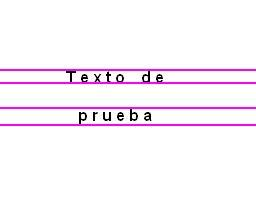
\includegraphics[scale=0.5,bb=0 0 256 203]{enmarcado1.png}
  \caption{ 1� delimitar las lineas del texto.}
\end{figure}

Ahora nos queda por saber cuales son las fronteras laterales para cada car�cter. El esquema anterior, para hallar los laterales no es �til cuando el mensaje ocupa mas de una l�nea, ya que en una l�nea puede haber un car�cter en la posici�n X donde en otra l�nea en esa posici�n X hay un espacio, por tanto considerar�a que en las dos l�neas hay un car�cter y en futuro se estudiara una regi�n que contiene un espacio creyendo que dentro hay un car�cter.

\begin{figure}[h]
  \centering
  
\includegraphics[scale=0.5,bb=0 0 256 203]{enmarcado2.png}
  \caption{ Este sistema fallar�a.}
\end{figure}

Es necesario realizar un barrido vertical de izquierda a derecha no para toda la imagen si no entre la coordenada Y superior y la inferior da cada una de las l�neas de caracteres antes calculada. As� iremos hallando las coordenadas X laterales izquierda y derecha para cada car�cter.

\begin{figure}[h]
  \centering
  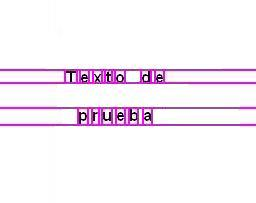
\includegraphics[scale=0.5,bb=0 0 256 203]{enmarcado3.png}
  \caption{ Sistema correcto.}
\end{figure}

Ya tenemos los datos mas importantes, ahora para definir un �rea rectangular solo es necesario guardar 2 coordenadas, por ejemplo la superior izquierda y la inferior derecha, por eso para cada car�cter utilizando los valores ya calculados le asociados 2 coordenadas que definir�n su �rea. Esta lista de pares de coordenadas ser� utilizada en la pr�xima funci�n de estudio de la morfolog�a del car�cter para que sepa que regiones de la imagen debe analizar.

\bigskip
Aun nos quedar�a un peque�o problema y es que dentro de una fila hay caracteres mas altos que otros, por ejemplo la 'o' es mas baja que la 'L', y para el posterior an�lisis nos interesa que las fronteras para cada car�cter est�n totalmente ajustadas a lo que realmente ocupa. Hay que reajustar las coordenadas de cada car�cter acerc�ndolas aun mas a este, este reajustamiento solo afecta a las coordenadas Y que son las que pueden estar desajustadas, el m�todo para ello es igual al utilizado para calcular los limites laterales. Ahora a partir de los limites laterales reajustamos para cada car�cter las fronteras superiores e inferiores.

\begin{figure}[h]
  \centering
  
\includegraphics[scale=0.5,bb=0 0 256 203]{enmarcado4.png}
  \caption{ Regiones de cada letra finalmente delimitadas.}
\end{figure}

Ya sabemos que regiones ocupa cada car�cter dentro de la imagen, sabemos que distancia existe entre cada regi�n. Esta informaci�n nos permite deducir si esa distancia es un espacio entre palabras o entre letras. Esto es muy �til ya que cuando a cada regi�n le asociemos un car�cter ASCII tendremos una lista de caracteres, pero no sabremos que palabras forman. Por ejemplo, si sabemos que entre el car�cter 6 y el 7 existe un espacio grande entre sus regiones esto ser� que el car�cter 6 y el 7 pertenecen a palabras distintas. 

Para esto hacemos la media aritm�tica de los espacios entre regiones contiguas sin contar las contiguas que est�n en distintas l�neas, aquellos espacios entre regiones que est�n por encima de la media ser�n espacios en blanco en el mensaje. Los espacios se representan como una cadena de booleanos de longitud igual al numero de regiones menos uno, que valdr� falso si entre dos regiones no se considera que exista espacio y cierto en caso contrario.

\subsection{Reconocimiento de patrones}
\subsubsection{Descripci�n}
Un reconocedor de patrones se puede considerar como un descriptor. Consiste en extraer caracter�sticas de un objeto para reconocerle.

\bigskip
Los descriptores se pueden clasificar en:
\begin{itemize}
\item Descriptores de frontera. (C�digos de cadena, n�meros de contorno, signaturas, ...)	
\item Descriptores de regi�n. (Descriptores globales, esqueleto de una regi�n, textura, momentos invariantes, ...)
\item Descriptores de estructuras tridimensionales.
\end{itemize} 
	
El algoritmo utilizado en el proyecto ha sido desarrollado por nosotros, se puede incluir dentro del �rea de descriptores de frontera. Ya que se basa en discriminar al objeto aprovechando las relaciones geom�tricas inherentes a la forma del objeto.
Definimos por tanto a un car�cter por su contorno.

\begin{figure}[h]
  \centering
  
\includegraphics[scale=0.5,bb=0 0 174 130]{letra.png}
  
\includegraphics[scale=0.5,bb=0 0 174 130]{letra1.png}
  \caption{ Caracter y su contorno.}
\end{figure}

El funcionamiento es el siguiente:
\begin{figure}[h]
  \centering
  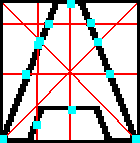
\includegraphics[scale=0.5,bb=0 0 140 143]{letra2.png}
  \caption{ Rectas que cortan al caracter en 12 puntos.}
\end{figure}

\begin{itemize}
\item Ajustamos un car�cter dentro de un marco.
\item Trazamos una serie de rectas que cortan al car�cter por varios puntos de su frontera. Estos puntos ser�n los que definir�n al car�cter. Seg�n el dibujo si trazamos 6 rectas conseguiremos 12 puntos para definir al car�cter.

\bigskip
Los puntos tienen que ser independientes de la posici�n que ocupa el car�cter dentro de la imagen en ese momento, tambi�n no tiene que importar el tama�o ya que un cartel podr� estar unas veces mas lejos que otras y una A siempre tendr� que seguir siendo una A independientemente de la distancia. Tambi�n en cierta medida el algoritmo tiene que ser permisivo con distintos tipos de formato.
\item Por eso, lo que se calcula es la distancia del segmento que se forma entre ese punto y el marco. No guardamos la distancia exacta, sino la proporci�n de la longitud del segmento con la de toda su recta. De esta forma ya no importara el tama�o de las letras, ya que aunque una A se mas peque�a q otra la proporci�n seguir� siendo la misma.

\begin{figure}[h]
  \centering
  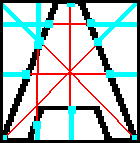
\includegraphics[scale=0.5,bb=0 0 140 143]{letra3.png}
  \caption{ Los 12 segmentos que definen al caracter.}
\end{figure}
\item Son entonces no 12 puntos lo que generamos sino 12 valores que indican la distancia relativa que hay desde esos puntos al marco. 
\item Para cada car�cter o digito calculamos sus 12 valores, y los guardamos en una base de datos junto con su identificador (car�cter ASCII).

As� tendremos en un archivo la descripci�n para cada car�cter en forma de 12 valores.

Ejemplo para 3 letras:

\textbf{A}  0.000000 30.882353 20.744681 20.744681 42.647059 26.470588 31.914894 31.914894 42.647059 26.470588 9.574468 9.574468 

\textbf{B}  0.000000 0.000000 0.000000 13.815789 0.000000 0.000000 0.000000 5.921053 2.941176 2.941176 0.000000 0.000000 

\textbf{C}  0.000000 0.000000 0.000000 85.227273 5.714286 5.714286 5.113636 5.113636 4.285714 4.285714 5.113636 1.704545 
\end{itemize} 

\subsubsection{Reconocimiento}
El reconocimiento es un proceso de etiquetado. se ocupa de identificar cada objeto segmentado de la escena y asignarle una etiqueta.

\begin{itemize}
\item Como todo modulo, el modulo OCR tiene su funci�n Iniciar, esta funci�n siempre cargara el archivo de descripciones en memoria para continuas consultas.
\item En cada ciclo cada vez que le llegue una imagen filtrada, el m�todo anterior llamado enmarcamiento de caracteres nos pasara en cada ciclo, una lista de N �reas o subimagenes q tendremos q tratar.
\item El ocr ira letra por letra (subimagenes) calculando sus 12 valores y compar�ndolos con los valores de las letras de la base de datos.
\item Aquel car�cter de la base de datos cuyos valores sean mas parecidos, es decir, generen menor error, ser� el que asignemos a esa subimagen. Es decir a cada subimagen se le asocia un car�cter ASCII.
\item As� con toda la lista de N subimagenes lo q generara una lista de N caracteres ASCII. Es decir una cadena de texto.
\item La funci�n anterior de enmarcamiento como dijimos infer�a por la distancia entre �reas si hab�a o no espacio entre letras, esta informaci�n se la pasa al reconocedor que la utiliza sobre la cadena de texto, poniendo o no espacios en blanco.
\item As� ya tenemos una cadena de texto formada por palabras. Palabras cuyas letras ser�n las que menos error han cometido seg�n el m�todo utilizado.
\end{itemize} 

Por tanto este m�todo asegura el reconocimiento de caracteres a distinto tama�o y en formatos distintos (no cursiva). 

La orientaci�n del mensaje se resuelve dentro del modulo de filtro anterior, con la funci�n de rotaci�n.

\subsection{An�lisis morfoLexico}
Muchas veces a causa del ruido del filtrado o por el formato de las letras, el OCR no asocia el car�cter ASCII correcto a la subimagen, por ejemplo puede confundir la letra 'N' con la 'H', ya que en algunos casos aunque lo que hayamos querido expresar en la imagen era una 'N' la 'H' genera menos error. 

Por este motivo ha sido necesario crear una ultima fase, que asegure la detecci�n y correcci�n de errores en el mensaje reconocido. Ya que a la salida de este modulo el mensaje ha de ser claro, para que robot pueda tratarlo ya sea como orden o como otra operaci�n.

\begin{figure}[h]
  \centering
  
\includegraphics[scale=0.4,bb=0 0 254 180]{dib_ana_morf.png}
  \caption{ Imagen recibida desde modulo filtro.}
\end{figure}
Para este ejemplo:

Frase reconocida por el OCR: ``TEXTO P8D58A''

Frase corregida por el analizador morfo-l�xico: ``texto prueba''

\bigskip
Esta ultima fase la forma una serie de funciones que componen el an�lizador morfo-l�xico del modulo OCR. Todo an�lisis morfo-l�xico se base en:
\begin{itemize}
\item Diccionarios (lexicones)
\item Reglas morfol�gicas
\end{itemize} 
Ambas cosas son interdependientes. Si en el diccionario s�lo guardamos lexemas, necesitaremos muchas reglas morfol�gicas.

Si guard�ramos todas las formas de las palabras en el diccionario, no necesitar�amos reglas morfol�gicas. Esto es lo que hemos seguido con nuestro diccionario, un diccionario con todas las formas verbales, etc.

Dificultades con los diccionarios:
\begin{itemize}
\item Polisemia: palabra con varios significados. Ej.: banco
\item Homonimia: palabras distintas con la misma graf�a. Ej.: divorciado: nombre, adjetivo y verbo
\end{itemize} 
Si fu�semos a hacer un tratamiento total del lenguaje natural del mensaje ser�a necesario que el diccionario fuese mucho mas completo, es decir, que guarde no solo las palabras si no mas informaci�n del tipo:
\begin{itemize}
\item Categor�a sint�ctica: preposiciones, conjunciones, nombre, adjetivo, verbo, etc.
\item Concordancia. G�nero, n�mero, persona, caso.
\item Preposiciones que admite un verbo, tipos de complementos, etc.
\item Informaci�n morfol�gica (patr�n de formaci�n de la palabra).
\item Informaci�n sem�ntica. Concepto correspondiente, palabras sin�nimas.
\end{itemize} 		
Los diccionarios se suelen organizar utilizando relaciones de herencia m�ltiple, tanto de tipo gramatical como conceptual.

Se implementan con tablas hash, tries o �rboles B. 

\bigskip
Nuestro diccionario no es tan complejo ya que solo act�a como verificador ortogr�fico.

Se organiza por bloques de palabras, cada bloque contiene palabras de la misma longitud, por tanto si la palabra mas larga en espa�ol contiene 23 letras, el diccionario posee 23 bloques, con palabras desde longitud 1 a longitud 23. Cada bloque es una tabla hash. 

La longitud de la palabra es algo en lo que se suelen cometer errores en el OCR, por tanto ya directamente buscamos la palabra de misma longitud, en un bloque determinado del diccionario. Si esta palabra no existe en la tabla hash solo se buscan palabras similares en un conjunto mucho mas restringido de palabras, que son las de su misma longitud.

\bigskip
Como ya hemos dicho el an�lisis en el modulo OCR no es demasiado amplio, esta parte entrar�a en el �mbito del modulo DCG. El OCR hace un an�lisis morfo-l�xico sencillo donde solo comprueba que las palabras del mensaje existen dentro del diccionario. Y en el caso de que no exista una palabra act�a de corrector ortogr�fico buscando la palabra del diccionario del mismo tama�o en letras que mas se aproxime a la palabra de la imagen, es decir, que seg�n el m�todo de reconocimiento del OCR menos valor de error genere.  

\bigskip
El error se calcula viendo los valores de los puntos que describen a cada car�cter de la palabra del diccionario en la base de datos del OCR, comparando la diferencia del valor de estos puntos con los obtenidos de su correspondiente car�cter asociado de la imagen, se va viendo cual de las palabras que realmente existen en el diccionario genera menos error. Recuerdo que la palabra que menos error genera seg�n este m�todo ser�a una secuencia de caracteres que no forman ninguna palabra existente. Por eso buscamos una palabra de mayor error, pero que exista. 

Este m�todo tiene un gran porcentaje de acierto entre el mensaje que representa la imagen y la que saca como salida el analizador.

\bigskip
Es por tanto el diccionario quien en ultima fase, pone la cadena de caracteres a la salida del modulo. Asegurando por tanto que todas las palabras que salgan de este modulo, son palabras que existen en el diccionario de espa�ol y que mas se corresponden con el mensaje del cartel.

\section{C�digo}
Ver HTML: documentaci�n del m�dulo en ocr.c y en ocr\_code.c.
%%% Local Variables: 
%%% mode: latex
%%% TeX-master: "vision"
%%% End: 

\chapter{M�dulo de Entorno 3D}

\section{Introducci�n}

El entorno virtual 3d constituye un interface visual con el usuario que puede observar la simulaci�n de las evoluciones de un robot que se desplaza por un escenario siguiendo las �rdenes procesadas por el sistema de visi�n por computador.

Con esta aplicaci�n, es posible evaluar y testar las funcionalidades que se han implementado sin tener que llegar a la integraci�n del sistema en una entidad rob�tica real.

\section{Detalles} 
\begin{itemize} 
\item {\bf Entrada}: Una estructura de datos que contiene una cadena de �rdenes y otra de par�metros.  
\item {\bf Salida}: Movimiento del robot virtual.
\item {\bf Descripci�n}: M�dulo que a partir de unas �rdenes representa el desplazamiento de un robot virtual a trav�s de un escenario en tres dimensiones.
\end{itemize} 


\section{Especificaci�n}

Para cumplir con su cometido, la aplicaci�n debe poseer las siguientes caracter�sticas funcionales:

\subsection{Representaci�n tridimensional de un entorno/escenario}

Teniendo en cuenta que una de las principales motivaciones para elaborar un sistema de �rdenes mediante visi�n artificial es la de implementar un dispositivo de navegaci�n que permita a un aut�mata desplazarse por su entorno, es fundamental simular gr�ficamente un escenario sobre el cu�l el robot virtual pueda desenvolverse. Esta representaci�n debe ser lo m�s inmersiva posible para que la precisi�n de la simulaci�n sea adecuada.
\subsection{Representaci�n de un robot capaz de desplazarse por su entorno}

Debe existir una entidad (en este caso un modelo 3D) dentro de la simulaci�n que represente la ubicaci�n, orientaci�n y desplazamientos resultantes de las distintas �rdenes procesadas por el sistema de control. Aunque en principio no es relevante, se ha intentando que esta entidad cumpla con ciertos criterios de dise�o que empaticen con los sistemas motrices m�s comunes en aut�matas (uso de ruedas, orugas, etc).
\subsection{Sistema de control}

Las diferentes �rdenes que son procesadas por el sistema de visi�n artificial, son analizadas para establecer las nuevas propiedades de posicionamiento, direcci�n, etc de la entidad que representa al robot. Esta interacci�n se realiza mediante el paso de mensajes distribuidos por el pipe que se encarga de la interconexi�n entre los diferentes m�dulos. Adem�s, es necesario que de forma aut�noma la aplicaci�n pueda procesar diferentes comandos emitidos por el usuario mediante el teclado y rat�n para poder controlar otros aspectos secundarios de la simulaci�n, como son el posicionamiento de la c�mara, activaci�n de diferentes efectos gr�ficos, etc.
 
\subsection{Sistema de c�maras interactivas}

Para poder visualizar de forma �ptima todos los componentes de la simulaci�n, es necesario poseer un sistema de c�maras que permita seguir c�modamente las evoluciones del robot por el escenario, as� como permitir al usuario adaptar la posici�n de las distintas c�maras para obtener el �ngulo de visi�n m�s relevante en cada momento.

\section{Implementaci�n}

La consecuci�n de las especificaciones previamente expuestas se ha conseguido mediante la implementaci�n de un amplio conjunto de caracter�sticas relacionadas principalmente con la programaci�n gr�fica 3D. A continuaci�n se describen detalladamente:

\subsection{Uso de DirectX 9.0}

La implementaci�n de los gr�ficos tridimensionales se ha realizada sobre la librer�a gr�fica Direct3D incluida en DirectX 9.0. Se ha optado por este est�ndar en vez del uso tambi�n muy extendido de la librer�a OpenGl por razones acad�micas, en el sentido de que previamente hab�amos tenido experiencia con OpenGl en otros proyectos y esta se presentaba como una oportunidad id�nea para investigar nuevas tecnolog�as. Cabe se�alar que ambas librer�as poseen similar potencialidad por lo que la elecci�n por razones funcionales no era especialmente relevante.
\subsection{Modelos 3D creados sobre 3dStudio Max 6.0}

Se ha empleado la herramienta de modelado 3dStudio Max para la elaboraci�n de los modelos tridimensionales tanto del escenario como del robot. Para su posterior integraci�n con la aplicaci�n, se ha utilizado un conversor que compatibiliza el formato usado por 3dStudio con el usado por Direct3D (archivos .X). En cuanto al apartado de las texturas, se ha utilizado Adobe PhotoShop para su realizaci�n.
\subsection{Terreno generado a partir de un mapa de altura}

Como parte del escenario, se ha incluido un terreno que es generado de forma procedural a partir de un mapa de altura. Una vez calculado la malla 3D de dicho terreno, se genera de forma procedural  la textura a partir de diferentes im�genes que se interpolan siguiendo como criterio la altitud del terreno. De esta forma, seg�n lo alto o bajo que est� el terreno, este presentar� el aspecto de diferentes materiales ( hierba para las zonas bajas, roca en las cumbres de las monta�as, etc). Por �ltimo se utiliza un algoritmo primitivo de sombreado que ilumina la textura resultante de forma coherente respecto a la posici�n de la luz en el escenario ( en este caso del sol).

\subsection{Iluminaci�n din�mica}

Para otorgar una mayor sensaci�n de integraci�n de la entidad que se desplaza con  el escenario, se ha utilizado iluminaci�n din�mica. De esta forma el robot es iluminado correctamente seg�n su posici�n actual, incrementando adem�s el realismo en la percepci�n de los materiales al visualizarse efectos de brillo, luz difusa, variaci�n crom�tica,etc.

 
\subsection{Iluminaci�n est�tica. LightMaps}

Los elementos est�ticos del escenario no requieren de iluminaci�n din�mica ya que su posici�n no var�a durante la ejecuci�n de la aplicaci�n. Para ahorrar recursos, es habitual el uso de texturas secundarias tambi�n llamadas lightmaps que codifican la informaci�n sobre la iluminaci�n que ese objeto recibe. En este caso, se ha utilizado una �nica textura resultado de la fusi�n de la textura primaria y los lightmaps para optimizar el rendimiento.

 
\subsection{Sombreado Din�mico. Stencil Buffer}

De forma an�loga a la iluminaci�n din�mica, el sombreado din�mico es un efecto que permite la integraci�n de objetos m�viles en escenarios de forma muy realista. Se ha implementado un algoritmo de sombreado que se basa en el uso del Stencil Buffer. Este algoritmo es bastante costoso en cuanto a recursos de la tarjeta gr�fica, por lo que sueles implementarse para ser soportado por tarjetas con aceleraci�n 3D de �ltima generaci�n.

\subsection{Luces Glow. Lens Flares}

Las luces Glow son puntos lum�nicos que producen un haz a su alrededor cuando se mira directamente. En este caso, se ha implementado un punto de luz que representa al sol. Adem�s, se ha implementado un efecto conocido como Lens Flares que se produce cuando se enfoca un sistema �ptico (c�mara de fotos, de video,etc) sobre un foco de luz intensa. Este efecto produce  una serie de reflejos residuales que se ubican de forma relativa a la luz que los origina. Se ha introducido por razones est�ticas y para incrementar la inmersi�n en el entorno virtual.

\subsection{Sistema de c�maras}

Se han implementando varios sistemas de c�maras para ofrecer m�ltiples posibilidades al usuario de seguir la acci�n que se desarrolla en la simulaci�n. Se dividen en:

\begin{itemize}

\item C�mara de seguimiento r�gido: La c�mara se sit�a siempre detr�s del robot y sigue cada uno de sus movimientos permaneciendo siempre a una misma distancia.

\item C�mara de seguimiento orbital: A diferencia de la anterior, esta c�mara orbita alrededor del robot manteniendo siempre su punto de enfoque fijado en �l.

\item C�mara fija: Se establece una posici�n de la c�mara donde permanece fija mientras enfoca y sigue los movimientos del robot.

\item C�mara libre: Con esta c�mara se puede navegar por todo el escenario as� como enfocar a los puntos de mayor inter�s para el usuario.
\end {itemize}

\subsection{Sistemas de part�culas}

De forma gen�rica, se ha implementado un sistema de part�culas para poder introducir efectos especiales y atmosf�ricos como pueden ser humo, fuego, lluvia, nieve, etc. Los sistemas de part�culas combinan una representaci�n gr�fica mediante billboards( pol�gonos especiales que mantienen siempre su orientaci�n respecto a la c�mara) y un sistema de control f�sico que determina el comportamiento de las part�culas en cuanto a aceleraci�n, direcci�n, tiempo de vida, turbulencia, etc.

 
\section{Dise�o}

El dise�o de la aplicaci�n es bastante sencillo en cuanto a su estructura jer�rquica. Existe una clase que contiene a la VentanaPrincipal de la aplicaci�n y que constituye el n�cleo de la ejecuci�n. Esta clase contiene un objeto del tipo Escena que es el que administra el resto de entidades con sus correspondientes representaciones gr�ficas. As�, la escena es el contenedor para otros objetos como son el Terreno, el Cielo, SistemaPart�culas, C�mara, y el resto de entidades como el escenario y el propio robot que pertenecen a la clase Objeto. Respecto a esta �ltima clase, destacar que posee como atributo un objeto de la clase Mesh que constituye la representaci�n gr�fica de la entidad (es decir, la maya 3d). Para gestionar la carga de los diferentes modelos 3d, existe una clase est�tica llamada MeshManager que comprueba que no se carguen en memoria varios modelos del mismo tipo. Por tanto, la creaci�n de objetos del tipo Mesh se realiza siempre a trav�s de esta clase gestora y nunca directamente. Por �ltimo, existen dos clases est�ticas que se encargan de la interacci�n del usuario mediante el rat�n y teclado ( clase Entrada) y otra que gestiona la impresi�n de texto en pantalla (clase Texto).

Respecto al flujo de ejecuci�n, se puede resumir en que existe un m�todo que es llamado externamente de forma peri�dica. Dicho m�todo hace que en cada ciclo se actualice la posici�n de cada uno de los objetos de la escena y posteriormente se renderice. Este proceso se hace de forma delegada, de forma que VentanaPrincipal llamar� al m�todo Render() de la Escena, la cu�l llamar� recursivamentea a los respectivos m�todos Render() de cada una de las entidades que contiene.

A continuaci�n se muestra un diagrama UML que de forma esquem�tica muestra las relaciones anteriormente descritas entre las principales clases que componen la apliaci�n:

\chapter{M�dulo de gesti�n de mensajes}

\section{Introducci�n}
Este m�dulo de la aplicaci�n tiene como misi�n recoger todos los mensajes que han podido ser generados por m�dulos de proceso anteriores, y filtrarlos de tal modo que la salida de la l�nea de ejecuci�n est� dotada de cierta coherencia con el resultado deseado. Para ello, admite las entradas en forma de cadenas de texto, y elige cu�les de ellas son las que deber�an dar realmente una salida a los m�dulos posteriores.

\section{Detalles}
\begin{itemize}
  \item {\bf Entrada}: Cualquier cadena de texto, y par�metros para controlar la tolerancia.
  \item {\bf Salida}: Una cadena de texto, la que m�s se asemeja a la que realmente deber�a ser generada.
  \item {\bf Descripci�n}: M�dulo que, a trav�s de la parametrizaci�n, guarda una tabla con las entradas, y, en funci�n de las cantidades de informaci�n, presenta la mejor salida.
\end{itemize}

\section {Arquitectura y funcionamiento del m�dulo}

El m�dulo trabaja con una \emph{tabla hash} inicialmente vac�a. Cuando recibe se�ales procedentes del m�dulo procesador, realiza una de las dos opciones siguientes:

\begin{enumerate}
\item \textbf{El elemento no estaba en la tabla}: Se a�ade a la tabla y se suma una unidad.
\item \textbf{El elemento ya estaba en la tabla}: Se suma una unidad al n�mero de llegadas consecutivas de ese elemento.
\end{enumerate}
Tras este primer paso, se procede a la ``debilitaci�n'' de las otras se�ales. Con esto queremos decir que reducimos el �ndice de refuerzo asociado a todas las se�ales que no fueran la que hemos escogido para que impere, tras una serie de ciclos que parametrizamos a trav�s de los argumentos del m�dulo, la se�al m�s importante (la que m�s veces seguidas ha llegado), que consideramos como la real que deber�a ser transmitida.

De esta forma, siempre mantenemos en la tabla todas las se�ales que van llegando, y creamos un tipo de diagrama de estados borroso, en el que el estado principal es decidido mediante los valores que el m�dulo va asignando a cada registro de la tabla.

Como utilidad a�adida, este m�dulo es uno de los m�s gen�ricos del \emph{pipeline}. El hecho de que los estados posibles se vayan creando de forma din�mica, y que sean s�lo diferenciados por una cadena de texto, ha hecho posible que el m�dulo sea usado para gestionar diferentes l�neas, sin tener que modificar ni una l�nea de c�digo. La �nica parte que hay que personalizar son los par�metros de la instanciaci�n del m�dulo, para que el comportamiento sea lo mejor posible.

?\chapter{M�dulo de control del robot}

\section{Introducci�n}
El m�dulo de control de robot ha sido creado con el fin de tener una pieza de software capaz de controlar nuestro robot de una forma sencilla y transparente para los m�dulos que generan la informaci�n de salida. A este m�dulo le llega una estructura de datos que contiene la orden y el par�metro, y el robot se encarga de moverse en funci�n de esa informaci�n. A continuaci�n detallamos c�mo lo hace.

\section{Arquitectura del m�dulo}
El m�dulo en s� tiene una estructura muy simple: consiste en un conjunto de funciones que son exportadas a un \emph{script} programado en el lenguaje \textbf{Lua}, y que funcionan principalmente haciendo llamadas a una librer�a que hemos creado, y que se encarga de controlar el puerto paralelo.

\subsection{Scripts}
La verdadera programaci�n de la funci�n del robot la hemos delegado en un \emph{script}. Este m�todo de programaci�n nos permite m�s flexibilidad a la hora de controlar el comportamiento de la m�quina.

En el script del robot implementamos algunas funciones determinadas que necesita el m�dulo de control, y las que nosotros deseemos. En este c�digo definimos de una manera muy simple qu� tiene que hacer el robot (realmente el puerto paralelo) cuando le llegan las �rdenes de los otros m�dulos.

\subsection{Biblioteca de control del puerto paralelo}
Hemos desarrollado una biblioteca que provee un interfaz lo m�s simple posible de control de los pines del puerto paralelo, y que adem�s es \textbf{multiplataforma}. A trav�s de ella se puede controlar los pines del cable, con llamadas simples, en las cuales s�lo hay que especificar que pin se quiere usar, y si se quiere poner a \emph{alta} o a \emph{baja}. De este modo nos hemos abstra�do, en la implementaci�n del m�dulo en s�, de las peque�as dificultades que puede ocasionar interactuar directamente con la entrada/salida del ordenador.

Para la implementaci�n de esta biblioteca hemos usado a su vez dos bibliotecas externas: \textbf{parapin} para la implementaci�n en GNU/Linux, y la DLL \textbf{inpout32.dll} para el uso en plataformas Win32.

\section{Construcci�n del robot}
Para construir la estructura f�sica del robot, hemos usado piezas de \emph{Lego Technics}. Este material es barato y razonablemente consistente para soportar su propio peso, el de la c�mara, el circuito, y el cable paralelo. Adem�s, destaca principalemente por su versatilidad de uso y su capacidad de reconstrucci�n. El ensamblado de las piezas es inmediato (hay que tener en cuenta que se vende como juguete para ni�os a partir de 12 a�os), y los errores de estructura se pueden subsanar con mucha facilidad.

Sin embargo, hemos escogido este material por la facilidad que hemos encontrado para generar m�quinas m�viles. Los conjuntos de piezas de \emph{Lego Technics} suelen venir acompa�ados por estructuras m�s complejas de construcci�n, como motores y brazos hidr�ulicos, elementos que hemos usado para nuestro robot.

El circuito ha sido conectado sobre una placa peque�a de entrenador, a pesar de su fiabilidad relativa, es r�pida de montar y de depurar. Hemos usado un chip \textbf{L293B}, que sirve para control de motores bidireccionales de corriente cont�nua, y alimentamos el circuito con una pila de 9 voltios. El circuito que usa el robot es el de la figura \ref{circuito_robot}.

%\usepackage{graphics} is needed for \includegraphics
%\begin{figure}[htp]
\begin{figure}[h]
\begin{center}
  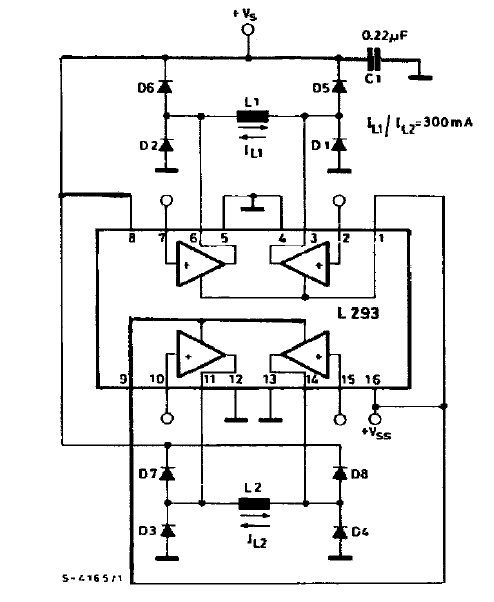
\includegraphics[scale=0.5,bb=0 0 494 602]{circuito.png}
  \caption{Cirtuito de control robot con chip \emph{L293B}}
  \label{circuito_robot}
\end{center}
\end{figure}

\section {Fotos}
A continuaci�n mostramos algunas fotos del robot que hemos construido:
% TODO: pues tud�

\begin{figure}[h]
  \centering
  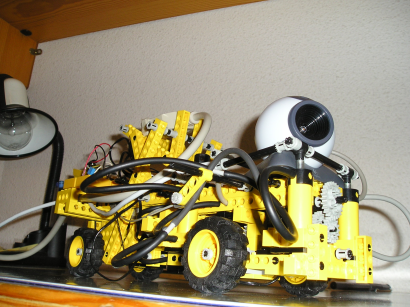
\includegraphics[scale=0.5,bb=0 0 410 307]{robot6.png}
% robot1.png: 72.009dpi, width=5.68cm, height=4.27cm, bb=0 0 161 121
  \caption{Foto lateral del robot}
\end{figure}

\begin{figure}[h]
  \centering
  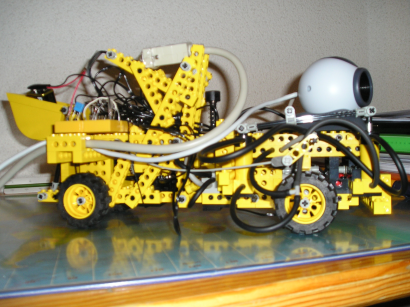
\includegraphics[scale=0.5,bb=0 0 410 307]{robot1.png}
% robot1.png: 72.009dpi, width=5.68cm, height=4.27cm, bb=0 0 161 121
  \caption{Foto inferior del robot}
\end{figure}





\section {C�digo}
% TODO: poner bien la referencia
Ver anexo: documentaci�n del m�dulo de robot.c, en \ref {robot_8c} (p�gina \pageref{robot_8c}).
\chapter{Procesamiento de texto reconocido}

\section{Introducci�n}
Una vez que el OCR ha reconocido una cadena de texto y la ha validado, env�a la se�al a este m�dulo, que se encarga de procesarlo, y crear una nueva salida en el formato propio del pipeline para el entorno 3D y el robot.

\section{Implementaci�n}

Para implementarlo, hemos usado un programa en \textbf{Prolog}, que est� formado en su mayor parte por una DCG \footnote{Definite clause grammar}. Este programa recibe la entrada del m�dulo, y, tras procesarla, crea una salida, que puede ser una cadena de respuesta, el resultado de una operaci�n aritm�tica (soporta par�ntesis y anidamiento de expresiones) o una orden para la salida.

\section{Ampliabilidad}

La idea de crear el m�dulo como antes hemos explicado ha sido propiciada por la idea de que la ``inteligencia del robot'' fuese algo ampliable. Con s�lo modificar este archivo, se puede dotar a la m�quina de m�s informaci�n (ampliando el diccionario), o de m�s capacidad de proceso (creando m�s reglas de reconocimiento en la DCG).

\section {C�digo}
% TODO: poner bien la referencia
Ver anexo: documentaci�n del m�dulo de prolog.c, en \ref {prolog_8c} (p�gina \pageref{prolog_8c}).
\chapter {Otros m�dulos}

\section{Introducci�n}
A continuaci�n explicamos el funcionamiento del resto de los m�dulos. Los aglutinamos en esta secci�n, por carecer de inter�s la explicaci�n detallada de los mismos, debido a su sencillez.

% TODO: poner las referencias

\section {M�dulo de post-gesti�n}
Hemos a�adido un m�dulo que recoja todas las se�ales que son generadas por las distintas ramas de proceso del \emph{pipeline}, y las agrupe en una sola salida v�lida, para ofrecer de este modo, a trav�s de sus puertos, datos a todos los m�dulos de salida.

Adem�s, hemos incluido en el m�dulo la posibilidad de generar salidas en un script, para que la depuraci�n de los m�dulos no dependa de los que est�n m�s arriba en el grafo, y tener m�s potencia de control de errores.

Puede examinar su documentaci�n de c�digo en \ref{caca}.

\section{Ventana de par�metros}
La ventana de par�metros es una interfaz gr�fica en la que es posible elegir un color, y tres tolerancias (una para el rojo, otra para el verde y otra para el azul), y alimentar as� a un m�dulo de filtro, de tal modo que la parametrizaci�n de los valores del mismo se pueda hacer en tiempo real.

Puede examinar su documentaci�n de c�digo en \ref{caca}.

\section{Ventana de im�genes}
La ventana de im�genes es simplemente un m�dulo que muestra gr�ficamente, en una ventana que se redimensiona autom�ticamente, una imagen que sigue el formato propio de nuestra aplicaci�n (ver secci�n \ref{formato_imagenes}).

La ventana de im�genes tiene como funci�n a�adida la capacidad de guardar una toma de la imagen que se este dibujando en el instante en el que se pulsa \textbf{F5}.

Puede examinar su documentaci�n de c�digo en \ref{caca}.

\section{M�dulo de control de joystick}
Hemos a�adido tambi�n al pipeline un m�dulo que, a trav�s de un interfaz de joystick, puede traducir sus entradas a las correspondientes �rdenes y par�metros del robot y del entorno 3D. De esta forma, la depuraci�n es sencilla y r�pida.

Para la implementaci�n hemos utilizado las bibliotecas SDL (Simple Directmedia Library).

Puede examinar su documentaci�n de c�digo en \ref{caca}.

\section{M�dulo de salida}
Este m�dulo es simplemente una ventana con un cuadro de texto que es capaz de imprimir en �l todas las cadenas (en formato C, \verb|char *|) que le llegan a trav�s de sus puertos.

Puede examinar su documentaci�n de c�digo en \ref{caca}.

\end{document}
